%\documentclass{emulateapj}
\documentclass[letterpaper,12pt,preprint]{aastex}

% packages
\usepackage{amssymb,amsmath,amsbsy}
\usepackage{booktabs}
\usepackage{bbold}
\usepackage{mathrsfs}
\usepackage{subfigure}
\usepackage[backref,breaklinks,colorlinks,citecolor=blue]{hyperref}
\usepackage[yyyymmdd]{datetime}
\renewcommand{\dateseparator}{-}
\usepackage{lscape}
\usepackage{rotating}

% commands
\newcommand{\given}{\,|\,}
\newcommand{\dd}{\mathrm{d}}
\newcommand{\transpose}[1]{{#1}^{\mathsf{T}}}
\newcommand{\inverse}[1]{{#1}^{-1}}
\newcommand{\mean}[1]{\left< #1 \right>}
\newcommand{\msun}{\ensuremath{\mathrm{M}_\odot}}
\newcommand{\bs}[1]{\boldsymbol{#1}}
\newcommand{\ident}{\mathbb{1}}
\newcommand{\inttime}{t_{\rm int}}

\newcommand{\project}[1]{\textsl{#1}}
\newcommand{\superfreq}{\project{SuperFreq}}

% TO DO
\newcommand{\todo}[2]{{\color{red} TODO: (\MakeUppercase{#1}) #2}}

\newcommand{\act}{J}
%\newcommand{\jac}{\bs{\rm J}}
%\newcommand{\jac}{\bs{G}}
\newcommand{\jac}{\mathscr{J}}

\begin{document}

\title{Chaotic mixing of tidal debris}
\author{Adrian M. Price-Whelan\altaffilmark{\colum,\adrn},
	    Kathryn V. Johnston\altaffilmark{\colum},
	    Monica Valluri\altaffilmark{\mich},
	    Sarah Pearson\altaffilmark{\colum},
	    Andreas H. W. K\"upper\altaffilmark{\colum},
	    David W. Hogg\altaffilmark{\nyu,\cds,\mpia}}
\date{\centering \today}

% Affiliations
\newcommand{\colum}{1}
\newcommand{\adrn}{2}
\newcommand{\mich}{3}
\newcommand{\nyu}{4}
\newcommand{\cds}{5}
\newcommand{\mpia}{6}
\altaffiltext{\colum}{Department of Astronomy, 
		              Columbia University, 
		              550 W 120th St., 
		              New York, NY 10027, USA}
\altaffiltext{\adrn}{To whom correspondence should be addressed: adrn@astro.columbia.edu}
\altaffiltext{\mich}{Department of Astronomy, 
			   University of Michigan,
			   Ann Arbor, MI 48109, USA}
\altaffiltext{\nyu}{Center for Cosmology and Particle Physics,
                      Department of Physics, New York University,
                      4 Washington Place, New York, NY, 10003, USA}
\altaffiltext{\cds}{Center for Data Science,
                      New York University,
                      4 Washington Place, New York, NY, 10003, USA}
\altaffiltext{\mpia}{Max-Planck-Institut f\"ur Astronomie,
                     K\"onigstuhl 17, D-69117 Heidelberg, Germany}

\begin{abstract}

% Context
The large-scale, smooth components of galactic gravitational potentials are thought to be triaxial in shape.
Triaxial potentials that match observational constraints and measurements of the radial profile and axis ratios of dark matter halos in cosmological simulations are almost certainly not globally integrable. 
An appreciable number of chaotic orbits are therefore expected in galactic halos.
It is yet unclear whether chaotic regions of phase-space will affect the density evolution of stellar tidal streams, which form in the halos of galaxies from the disruption of stellar systems.
% Aims
Many numerical methods exist for assessing the degree of chaos for a given orbit (e.g., the Lyapunov exponent, the frequency diffusion rate). 
These indicators, which are local to a single orbit, often predict a timescale over which chaos will be dynamically important.
In this paper, we aim to compare these timescales to the density evolution of the finite-volume ensembles of orbits.
% Methods: 
We derp derp derp.
% Results:
We find that mean indicators such as the Lyapunov time or the (long term) frequency diffusion rate of a given ``parent'' orbit are not good predictors for the short-term density evolution of ensembles of orbits around this parent orbit.
Instead, we find that the variance of the fundamental frequencies of the ensemble orbits over short timescales is a stronger indicator of the density evolution.
% Conclusions:


\end{abstract}

\keywords{
}

\section{Introduction}\label{sec:introduction}

The dark matter halos of galaxies are thought to be triaxial in shape. However, despite suggestive evidence from a range of complimentary observational methods, this fundamental prediction from $\Lambda$CDM cosmology has not been conclusively verified. Around other galaxies, it is generally hard to measure the 3D mass profile because they are seen in projection. From the Earth's position within the Milky Way, our view of our own halo and proximity gives us a unique chance to directly measure the 6D positions of stars and model the shape of the mass distribution at large radii. The Milky Way halo has a low density of visible tracers, but luckily many of the halo stars are likely on non-random orbits and thus contain extra information (e.g., debris stripped from stellar systems).

As a satellite galaxy or globular cluster orbits within some larger system, mass is eroded due to the tidal forces of the host galaxy potential. If the orbit of such an object is regular, only mildly eccentric, and stays far from sharp density features (e.g., the disk), the disruption is a steady process and the mass is slowly stretched into long streams of matter known as stellar tidal streams. The phase-space density and therefore the observable properties of these tidal streams are sensitive to the internal progenitor properties, orbit of the progenitor, and mass distribution of the host galaxy. Many tidal streams are observed around the Milky Way, M31, and other nearby galaxies that span a large range of distances \citep[$\approx$10--100~kpc][]{cite many}. The morphological evolution of tidal debris depends on the spread of orbital properties (e.g., actions or frequencies) of the debris and the orbit of the progenitor system, both of which are also determined by the shape and radial profile of the gravitational potential of the host galaxy. By simultaneously modeling the observed phase-space density of stream stars along with the potential, it is hoped that we may infer the dark matter distribution around the Milky Way.

Tidal streams are generally modeled as 1D structures formed on regular orbits with simple internal progenitor dynamics and density evolution. Methods span a range of complexity from orbit-fitting, to \emph{Streakline} or particle-spray models, to action-space density modeling, to N-body simulations \citep[see, e.g., the introduction of][]{kuepper15}. All methods have been tested in some way on simulated observations of data and these tests typically demonstrate the recovery of parameters for analytic, static potential forms. Many of the methods have been shown to work in axisymmetric or otherwise simple potentials but may extend to more complex, generalized potentials (e.g., triaxial or multi-component potentials). 

One example of stream modeling in a multi-component (static, analytic) potential was done by \citet{pearson15}, who tried to reproduce observations of the stellar stream density from the globular cluster Palomar 5 in a single oblate and single triaxial potential using \emph{Streakline} \citep{kuepper12} and N-body models. They use the observed SDSS number density of stream stars, a limited number of radial velocities for stream members, and the sky position, distance, radial velocity, and proper motion of the cluster itself to fit model streams to the data. In the oblate potential (a three-component bulge+disk+spherical halo potential), a thin model stream is easily found that reproduces the observed stellar density morphology of the stream. In the triaxial potential (the potential from \cite{law10}: a three component bulge+disk+triaxial halo fit to Sagittarius stream data), the model streams generically form large, two-dimensional ``fans'' of debris near the ends, and there are no physically reasonable progenitor orbits that reproduce the observed thinness of the stream given the observational constraints of the present-day position and velocity of the cluster. 

The obvious difference between the two potentials considered by \citet{pearson15} is the extra symmetry of the triaxial potential. It is well known that the number of degrees of freedom of a potential plays a critical role in determining the orbit structure of the potential --- Hamiltonians with more than two degrees of freedom generically contain significant chaotic regions. \citet{pearson15} tested the stochasticity of the orbit of the progenitor that produced fanned debris by computing the Lyapunov exponent along this orbit but found that it is consistent with being regular over dynamically relevant timescales (many Hubble times). It has been shown previously that along some strongly chaotic orbits, tidal streams do form large, diffuse fans of debris \citep[e.g.,][]{fardal14}, however it is unknown how the resultant properties of the debris (e.g., density or length of the stream) depend on the degree of stochasticity. The result from \citet{pearson15} suggests that even weak chaos (as measured by the Lyapunov exponent) may affect the density evolution and therefore observability of tidal streams. 

In this work, we study the effect of chaotic diffusion on tidal stream morphology. We choose a simple, cosmologically motivated model for a triaxial potential, analyze the degree of chaos as computed from single-orbit diagnostics for grids of constant-energy orbits, and compare these results to measures of the density evolution of finite-volume ensembles of orbits (meant to mimic tidal debris). We find that even when the chaotic timescale is predicted to be long for a given orbit, chaos may manifest over much shorter times in small orbit ensembles due to the nature of chaotic diffusion. This result supports a reevaluation of the importance of chaos in galactic halos and implies that the amount of chaos in a given potential may have significant consequences for the observability and survivability of thin, cold tidal streams. 

This paper is organized as follows. We review relevant nonlinear dynamics in Section~\ref{sec:nldreview}. In Section~\ref{sec:methods}, we describe our choice of potential, method for numerical orbit integration, and introduce the chaos indicators used in this work. Our results are split into three subsections: in Section~\ref{sec:results1} we present iso-energy grids of orbits and discuss the orbit classes and chaotic timescales present in our potential; in Section~\ref{sec:results2} we study the density evolution of small ensembles of orbits around each orbit of the previous section; and, in Section~\ref{sec:results3} we describe the behavior of chaotic diffusion and use this to explain how chaos is relevant for tidal streams over short times. We discuss the implications of our results in Section~\ref{sec:discussion}, and conclude in Section~\ref{sec:conclusions}.

\section{Review of nonlinear dynamics}\label{sec:nldreview}

In order to explore the question of how chaos manifests over timescales much shorter than that predicted from generic chaos indicators, we must first understand the structure and behavior of orbits in complex gravitational potentials. An orbit in an $N$ degree of freedom (dof) Hamiltonian, $H$, is a set of $2N$ quasi-periodic time series, 
\begin{equation}
(w_1(t),...,w_{2N}(t)) = (q_1(t),...,q_{N}(t),p_1(t),...,p_{N}(t)) \label{eq:coords}
\end{equation}
where $q_i$ and $p_i$ are conjugate coordinates in the sense that
\begin{align}
	\dot{p}_i &= -\frac{\partial H}{\partial q_i}\\
	\dot{q}_i &= \frac{\partial H}{\partial p_i}
\end{align}
for all $t$. If bounded, the motion in any component, $w_i(t)$, can be represented as a Fourier sum,
\begin{equation}
	w_i(t) = \sum_k^\infty a_k \, e^{i\,\omega_k\,t} \label{eq:fourier}
\end{equation}
where the $a_k$ are complex amplitudes.

A \emph{regular orbit} is a set of such time series that can be transformed to a special set of canonical coordinates known as angle-action coordinates. In these coordinates, the position variables are angles, $\boldsymbol{\theta}$, that increase linearly with time with rates set by $N$ constant, fundamental frequencies, $\boldsymbol{\Omega} = (\Omega_1, ..., \Omega_N)$. The frequency of a Fourier component in the sum for any individual component of motion (the $\omega_k$ in Equation~\ref{eq:fourier}) are just linear, integer combinations of the fundamental frequencies, $\boldsymbol{\Omega}$ --- that is, for a regular orbit, any Fourier component frequency may be written
\begin{align}
	\omega_k &= \boldsymbol{n_k} \cdot \boldsymbol{\Omega} \label{eq:fourierfreq}
\end{align} %; \, (\boldsymbol{n}_k \in \mathbb{Z}^3)
where $\boldsymbol{n}_k$ is a vector of $N$ integers. The conjugate momentum coordinates --- the actions,  $\boldsymbol{J}$ --- are constants of motion. Even stronger, the actions are isolating integrals and any pair are in involution such that
\begin{equation}
	[J_i, J_j] = 0
\end{equation}
where $[\cdot,\cdot]$ is the Poisson bracket. This implies that for an $N$ dof system, a regular orbit has $N$ independent constants of motion and the motion is therefore restricted to an $N$-dimensional manifold embedded in the 2$N$ dimensional phase space. The topology of angle-action space is toroidal and any regular orbit in an $N$ dof Hamiltonian can be understood as motion on the surface of an $N$-torus. Each set of actions, $(J_1,...,J_N)$ (or frequencies), uniquely labels a torus, and regular orbits are sometimes referred to in terms of their orbital tori. 

\subsection{Orbits in integrable potentials}

A Hamiltonian or potential is said to be \emph{globally integrable} when the number of isolating integrals of motion is equal to the number of degrees of freedom and a transformation to angle-action coordinates may be done globally --- for example, the transformation to angle-action coordinates may be written as a function of arbitrary phase-space coordinates and the functional form is independent of phase-space position. The condition for global integrability is very restrictive and it seems that the likelihood that a Hamiltonian is globally integrable decreases as the number of degrees of freedom increase \citep[e.g.,][]{lichtenberg83}. In a globally integrable potential, the Hamiltonian may be written solely in terms of the actions, $H = H(\boldsymbol{J})$. Galactic potentials are almost certainly not globally integrable, but it is useful to understand the orbit structure in integrable systems before extending to more general potentials. Only one globally integrable triaxial mass model is known that generates motion that is qualitatively similar to that seen in Galaxies: the St\"ackel or ``Perfect Ellipsoid'' model \citep[e.g.,][]{kuzmin73, deZeeuw85}. The four general classes of orbits in this potential are box, inner long-axis tube, outer long-axis tube, and short-axis tube orbits. The tube orbits preserve a sense of rotation about either the long or short axis and are therefore centrophobic, whereas the box orbits may approach arbitrarily close to the center of the potential (centrophilic) and may change the sense of rotation about any axis.

The frequencies of a generic, non-resonant orbit are incommensurable --- that is, $\bs{n} \cdot \bs{\Omega} \neq 0$ for any integer vector, $\bs{n}$, with reasonable magnitude.\footnote{A more precise condition is stated in terms of a diophantine condition, e.g., $|\bs{n} \cdot \boldsymbol{\Omega}| > \alpha \, |n|^{-\gamma}$ where $\alpha, \gamma>0$.} These conditionally-periodic orbits uniformly cover the surface of an orbital torus. If instead there exists a relation of the form $\boldsymbol{n} \cdot \boldsymbol{\Omega} = 0$ the orbit is a resonant orbit. For resonant orbits, the existence of an additional \emph{local} constant of motion reduces the dimensionality of the orbit. We refer to orbits that obey a single resonance relation as \emph{uni-resonant} orbits, and if an additional resonance relation exists, \emph{bi-resonant}. The resonant structure of a potential --- the relative importance of particular resonance numbers --- is difficult to compute, but determines the global behavior of orbits in the potential. For a triaxial potential the resonances define planes in frequency-space, but resonance surfaces in action-space are generic 2D surfaces. In plots of frequency ratios, the resonances appear as lines; Figure~\ref{fig:cartoons} (left panel) shows a cartoon portrait of a portion of frequency-space for an integrable potential with resonance lines, non-resonant, and resonant orbits marked. For an integrable potential, all non-resonant orbits are regular.

\subsection{Orbits in near- and non-integrable potentials}

The orbit structure of near-integrable potentials can be understood by considering a Hamiltonian that is a small perturbation away from being globally integrable --- that is, a Hamiltonian that may be written
\begin{equation}
	H(\boldsymbol{J}, \boldsymbol{\theta}) = H_0(\boldsymbol{J}) + \epsilon \, H_1(\boldsymbol{J}, \boldsymbol{\theta})
\end{equation}
where $H_0(\bs{J})$ represents an integrable Hamiltonian, and $\epsilon$ is a small parameter that determines the perturbation strength \citep[a complete description of perturbation theory applied to nonlinear Hamiltonians is given in][]{lichtenberg83}. When $0 < |\epsilon| \ll 1$, resonant surfaces become ``thick'' resonant layers, within which orbits are qualitatively similar to the parent resonant orbit \citep[e.g.,][]{merritt99}, and these layers regions are then generically surrounded by stochastic layers where chaotic motion occurs. Chaotic orbits are characterized by exhibiting random behavior despite being generated by entirely deterministic equations of motion. Stochastic layers form gaps in action space where tori are destroyed; the orbits that exist in these regions therefore can not be represented in angle-action coordinates, as their actions and frequencies are not constant and diffuse chaotically with time. 

Figure~\ref{fig:cartoons} (middle panel) shows a cartoon of frequency space for a near-integrable potential (a small perturbation away from the potential in the left panel). Much of the structure that was present in the integrable potential remains in the near-integrable case, but the differences are highlighted. Orbits in the resonant layers surrounding the resonances (grey) are near-resonant orbits that will librate around the resonance. Chaotic orbits in the stochastic layer (red) behave erratically depending on the surrounding resonance structure. If the stochastic layer is small and the chaotic orbit is therefore confined in some way, it may behave nearly regular for long periods of time.

For small values of $\epsilon$, many regular orbits survive and only small chaotic regions are introduced, especially where resonances overlap. As the strength of the perturbation increases, eventually all tori associated with conditionally-periodic motion will be destroyed. Figure~\ref{fig:cartoons} (right panel) qualitatively shows this phenomenon --- the resonant and resonant-layer orbits may still be regular, but many or all of the conditionally-periodic orbits can be chaotic. As the perturbation strength increases, next the uni-resonant tori are destroyed, and finally the bi-resonant tori --- these are least susceptible to destruction from perturbations \cite[for a more quantitative illustration of this transition from integrability to global chaos, see Figure~9 in][]{valluri98}.

When $\epsilon$ is large, there is no general prediction for the resulting behavior, however it seems that more complicated and physically motivated triaxial potential models for galaxies follow the intuition gained from the small-perturbation picture described above, at least for certain parameter choices \citep{valluri, merritt, dehnen, etc.}. We therefore expect a large number of regular orbits will survive --- the so-called KAM tori --- however the tori that survive will be separated by regions of chaotic motion. Any transformations to angle-action coordinates must be defined locally due to the destruction of tori caused by the onset of chaotic motion. 

\subsection{The behavior of chaotic orbits in non-integrable potentials}\label{sec:behavior-chaotic}

Chaotic orbits have no orbital actions because they are only strictly bound to their energy hypersurface (if the potential is time-independent). The orbits therefore do not have a single set of fundamental frequencies, but rather the frequencies that describe the character of motion evolve with time. In near-integrable potentials, chaotic diffusion of an orbit in actions and frequencies occurs both across resonance layers (a sort of stochastic libration) and along the stochastic layers that surround the resonances (Arnold diffusion). For weakly chaotic orbits, motion across a resonance layer can occur with a frequency close to the libration frequency of the nearby stable orbits in the resonance layer. Thus, if the resonance libration frequency is comparable (within a factor of a few) to the orbital frequency, motion across a resonance can modulate the frequency spectrum of an orbit over dynamically relevant timescaes. However, the stochastic layers are often bounded in the direction orthogonal to the resonance by other stable, resonant regions so that the frequencies or actions can't change by large factors (unless there is resonance overlap and the motion is strongly chaotic). The rate of diffusion along stochastic layers via Arnold diffusion depends on the local resonant structure and is hard to predict, however, this has been done analytically for simple potentials \citep[e.g.,][]{chirikov??}. For systems with $N>2$ dof, the stochastic layers connect and form an intricate network of stochasticity known as the Arnold web; an orbit that ergodically mixes over its energy hypersurface must traverse this web, though the timescales typical for this phenomenon are many thousands of orbital periods.

Small ensembles of (conditionally-periodic) regular orbits will reach a fully phase-mixed state in a timescale  $\approx\sigma_\Omega^{-1}$, where $\sigma_\Omega$ is the dispersion in frequency-space of the ensemble --- each individual orbit will fill the surface of its torus ergodically, but the ensemble will only mix due to sheering from slight variations in their fundamental frequencies \citep{merritt96, helmi99}. Ensembles of chaotic orbits behave quite differently. Over long times, a chaotic orbit in an autonomous Hamiltonian will ergodically mix over the energy hypersurface (a 5D surface, compared to the 3D stable tori). Generically, a small ensemble of chaotic orbits will lose coherence much faster than for regular orbits, however analytically computing the rate and amount of spreading is very difficult even for simple potentials \cite[see, e.g.,][]{chirikov??}. Certain ensembles may be trapped between resonances for long times and thus remain in a state of pseudo-coherence for long times, whereas others may rapidly diffuse \citep[see, e.g.,][]{merritt96}. This phenomenon is generic to potentials that are not globally stochastic in which regions of stability and chaos are intermingled throughout phase-space. 

\todo{apw}{concluding paragraph...}

\section{Numerical methods}\label{sec:methods}

Our goal is to map the orbit structure of arbitrary potentials, with an emphasis on identifying the chaotic orbits and and understanding the evolution of these orbits over short times. In this section, we describe the methods we will use to detect and quantify the strength of chaos for large grids of orbits.

\subsection{Potential choice}\label{sec:potential}

The density distributions within dark matter halos formed in cosmological N-body simulations are generically triaxial \citep[e.g.,][]{jing02, bett07, zemp09, veraciro11}. With the inclusion of baryonic physics and sub-grid prescriptions for energy input due to supernovae and other feedback mechanisms, the inner potential ($\lesssim$$0.1R_{\rm vir}$ for a $\approx$$10^{12}~\msun$ halo mass) typically becomes more spherical, though the magnitude of this reshaping depends on the particular merger history and star formation efficiency within a given halo \citep[e.g.,][]{dubinski??, butsky15}. It is less clear what happens to the outer halo where tidal streams are more readily found. %; for this reason, we ask what we would expect to happen to tidal streams if the halo in which they form is strongly triaxial.

 \citet[][hereafter JS02]{jing02} found that a triaxial generalization of the NFW density profile \citep{navarro96} generates excellent fits to the density distributions within haloes in their high-resolution N-body simulations, and they provide probability distributions for the axis ratios of a large sample of these halos. JS02 finds median axis ratios of $c/a \approx 0.55$ and $b/a \approx 0.77$ where $a$ is the major axis, $b$ the intermediate, and $c$ the minor axis.\footnote{Note that JS02 use the opposite notation so that $c$ is the major and $a$ is the minor axis.} These are largely consistent with findings from more recent simulations \citep[e.g.,][]{millenium, hmm, butsky15} and consistent with constraints from weak lensing that place a lower limit on minor-to-major axis ratios of $c/a\gtrsim0.5$ \citep{vanuitert12}. JS02 finds significant scatter in the distributions of concentration parameter, $c_e$, or scale radius (depending on choice of parametrization). 

All of these parameters are specified in terms of the \emph{density}; for orbit analysis, we need to determine the form of the potential in terms of these parameters, which, in general, requires numerical integration of the density at each position of interest. For computational efficiency, many authors instead express the triaxiality in the form of the potential, but this can lead to unphysical situations where the density becomes negative. \citet{leesuto03} derive a perturbative expansion of the potential integral for a triaxial NFW density and show that the expansion is accurate even for modest axis ratios (e.g., the median values shown above). 

In this work, we use the triaxial potential expression from \citet{leesuto03}, parametrized in a slightly different manner. In terms of spherical coordinates\footnote{$(r,\phi,\theta)$ = (radius, azimuth, colatitude)} with the radius normalized by the scale radius, $u = r/r_s$
\begin{align}
	\Phi(u,\phi,\theta) &\approx \frac{v_c^2}{A}\left[F_1(u) + \frac{1}{2}(e_b^2 + e_c^2)F_2(u) + \frac{1}{2} [(e_b\sin\theta \sin\phi)^2 + (e_c\cos\theta)^2] F_3(u) \right]\label{eq:potential}\\
	A &= \left(\ln2 - \frac{1}{2}\right) + \left(\ln2-\frac{3}{4}\right) (e_b^2 + e_c^2)
\end{align}
where $e_b = \sqrt{1 - (b/a)^2}$, $e_c = \sqrt{1 - (c/a)^2}$, and $v_c$ is the circular velocity at the scale radius, $r_s$, for the spherical case. The functions $F_i(u)$ are given in the appendix of \cite{leesuto03}. We chose $r_s=20~{\rm kpc}$ and $v_c = 175~{\rm km}~{\rm s}^{-1}$ by taking the mean halo concentration for a ${\rm M}_{vir} \approx 10^{12}~\msun$ halo, $c_e\approx5$, from \cite{jing02} and by assuming $R_{vir}\approx200~{\rm kpc}$. Figure~\ref{fig:potential} shows equipotential contours of this potential in projection, and Table~\ref{tbl:potential} summarizes the potential parameters.

\begin{table*}[ht]
\begin{center}
	\begin{tabular}{ c  c }
	         Parameter & Value\\\toprule
		$v_c$ & 175~km~s$^{-1}$\\
		$r_s$ & 20~kpc\\
		$a$ & 1\\
		$b$ & 0.77\\
		$c$ & 0.55\\
		\bottomrule
		\end{tabular}
	\caption{Summary of potential parameters for the triaxial NFW potential (Equation~\ref{eq:potential}) used in this work. Triaxiality is introduced in the density to ensure the density is physical at all radii. Velocity scale, scale radius, and axis ratios are chosen to match the median halo parameters for a $M_{\rm vir} \approx 10^{12}~\msun$ halo from \citep{jing02}. \label{tbl:potential}}
\end{center}
\end{table*}

This potential is a simple and unrealistic model for the total potential of a Milky-Way-like galaxy, however it represents a conservative choice for exploring the structure of orbits in the halos of such galaxies. Realistic galactic potentials will have a significant component due to the disk and bulge, may have twisting inertia tensors \citep{romanowsky98}, radially changing axis ratios \citep[e.g.,][]{kazantzidis04,debattista08,veraciro11,butsky15}, significant substructure \citep{moore98,zemp09}, or time dependence \citep[either from bulk rotation, mass growth, mergers, etc.; see, e.g.,][]{bailin05}. We expect inclusion of any of these effects to increase the amount and influence of chaos; see the Discussion (Section~\ref{sec:discussion}) for a few simple demonstrations. \todo{apw}{Cite this paper: hunter05 for disk crossings and chaos}

\subsection{Orbit integration}\label{sec:integration}

We use the Dormand-Prince 8th-order Runge-Kutta scheme \citep{prince81} to integrate orbits in the above potential. Specifically, we use a \texttt{Python} wrapper over the \texttt{C} implementation by \cite{hairer93}. For all orbits we ensure that energy is conserved to $|\Delta E/E_0| \leq 10^{-8}$ by the end of integration, however most orbits conserve energy to a part in $\approx$$10^{-13}$. Unless otherwise specified the integration timesteps are chosen so that there are 512 steps per strongest orbital period component, but the integrator uses adaptive stepping between each main step in order to satisfy a specified tolerance (we set the absolute tolerance to $\approx$100 times machine precision, $\texttt{atol} = 10^{-13}$). 

\subsection{Lyapunov exponents} \label{sec:lyap}

The most well-known method for assessing chaotic motion is to analyze the Lyapunov spectrum or maximum Lyapunov exponent (MLE) of an orbit. The MLE measures the mean rate of divergence of two infinitesimally separated orbits and is only strictly defined in terms of a limit that goes to infinite time. Thus, we can never truly compute the MLE and it can take integration for many thousands of orbital periods to compute a converged numerical approximation of the MLE for a moderately chaotic orbit. In this work, we use the algorithm introduced by \cite{wolf85} for computing the MLE (for more a more detailed description of this algorithm, see Appendix~\ref{sec:lyapapdx}).

The MLE, $\lambda_{\rm max}$, is interpreted as a rate that sets the exponential divergence of infinitesimally close chaotic orbits. It is therefore useful to consider the corresponding $e$-folding time, 
\begin{equation}
	t_{\rm \lambda} = \frac{1}{\lambda_{\rm max}}.
\end{equation}
We will use this as the prediction from the Lyapunov exponent for the timescale over which chaos should be dynamically important for a given orbit. 

\subsection{Frequency diffusion rate}\label{sec:naff}

Bounded, regular orbits in a triaxial potential have three fundamental frequencies, $\bs{\Omega}$, that determine the periodic behavior of motion. The motion in any canonical coordinate can therefore be decomposed as a Fourier sum (Equation~\ref{eq:fourier}) where the Fourier frequencies are linear, integer combinations of the fundamental frequencies (Equation~\ref{eq:fourierfreq}). \cite{laskar93} introduced a method for recovering the fundamental frequencies of an orbit that effectively uses a Hamming-filtered fast-Fourier transform (FFT) of complex combinations of the motion (e.g., $x(t) + i v_x(t)$). It has been shown that using a filtered FFT makes the accuracy in determining the frequencies converge much faster than the typical $\inttime^{-1}$ expected for a standard FFT \citep{laskar99}, where $\inttime$ is the integration time. The FFT is iteratively searched for the strongest frequency component, which is subtracted from the spectrum after each iteration. This procedure generates a table of frequencies for each component of motion which must then be searched for the three fundamental frequencies.

This method is referred to as ``Numerical Approximation of Fundamental Frequencies'' (NAFF) and has been used extensively in planetary dynamics \citep[e.g.,][]{laskar93b, laskar96} and galaxy dynamics \citep{papaphilippou98, valluri98}, especially in the study of orbits in triaxial systems. We have implemented and tested a version of this procedure in the \project{Python} programming language. Our implementation differs slightly from the original definition and from that used in \cite{valluri98}: we have found that using a higher order window function \citep[e.g.,][]{hunter02} of the form
\begin{equation}
	W(t/\inttime) = \frac{2^p \, (p!)^2}{(2p)!} \left( 1 + \cos \frac{\pi t}{\inttime}\right)^p
\end{equation}
with $p=2$ allows for more reliable determination of frequencies from strongly chaotic orbits. We refer to this slight modification of the algorithm as \superfreq\ and the code is open-source and publicly available on \project{GitHub} at \url{https://github.com/adrn/SuperFreq}. For more details about the algorithm, see Appendix~\ref{sec:naffapdx} or \cite{laskar88, laskar93, papaphilippou96}.

If an orbit is chaotic, the motion can no longer be expanded in terms of a single set of fundamental frequencies. For a weakly chaotic orbit, the orbit may appear consistently periodic over long windows of time. \superfreq\ will pick out a set of frequencies for such orbits that correspond to the largest peaks in the power spectrum of the stochastic orbits, however these peaks will change location and amplitude with time. For more strongly chaotic orbits, the power spectrum will be quite noisy and the peak frequencies may change erratically when comparing two separate sections of orbit. The frequencies picked out by \superfreq\ for such orbits will therefore represent the average periodic nature of the orbit over a given period. We define the fractional frequency diffusion rate per orbital period, $\mathcal{R}$, in the $i$th fundamental frequency as
\begin{equation}
	\mathcal{R}_i = \frac{\Omega_i^{(2)} - \Omega_{i}^{(1)}}{\Omega_{i}^{(1)} \, N} \label{eq:fdrate}
\end{equation}
where $\Omega_i^{(1)}$ and $\Omega_i^{(2)}$ is the $i$th fundamental frequency computed in each of two consecutive sections of orbit and $N$ is the number of orbital periods in a single section of orbit. By inverting this rate, we can compute the timescale over which we expect order-unity changes to the fundamental frequencies: the \emph{frequency diffusion time} is defined as
\begin{equation}
	t_\Omega = \, (\max_{a_i} \, \mathcal{R}_i)^{-1} \label{eq:fdtime}
\end{equation}
where the maximum is taken with respect to the corresponding amplitudes, $a_i$, of the fundamental frequency components \citep[see][]{valluri12}, and the time is in units of number of orbital periods, ${\rm T}$. For a small ensemble of orbits (e.g., tidal debris), the relevant timescale is the time over which the change in frequencies for a single orbit is comparable to the spread of frequencies in the ensemble. We can estimate this timescale by multiplying the frequency diffusion time by a factor equal to the fractional spread in frequencies of the debris. For example, a globular cluster typically has $\approx$1\% spreads in fundamental frequencies, so by multiplying the frequency diffusion time by $f = 0.01$, we can estimate the time (number of orbital periods) over which we expect the frequencies to evolve by this amount.

% =====================================================================
%	Results
%
\section{Results}

In Section~\ref{sec:results1}, we generate grids of orbits in the potential described above to map the orbit structure of the potential. We classify each orbit in terms of the strength of chaos along the orbit as computed using the methods of Section~\ref{sec:methods}. With this initial classification, in Section~\ref{sec:results2} we follow the evolution of ensembles of orbits generated around each orbit in the initial grid. We find that the configuration-space density of ensembles around weakly chaotic orbits evolve faster (e.g., in mean density) than expected given the timescales over which chaos is computed to be relevant for the parent orbits. In Section~\ref{sec:results3}, we explain this phenomenon in the context of how chaotic diffusion occurs (e.g., Section~\ref{sec:sec:behavior-chaotic}).

\subsection{Part I: Lyapunov and frequency diffusion times}\label{sec:results1}

We generate isoenergy grids of initial conditions along the $xz$ ($y=0$) plane\footnote{$x$ is the major and $z$ the minor axis.} with energy (per unit mass) chosen to span a range of distances comparable to the scale radius of the potential ($E=-(397.2~{\rm km~s}^{-1})^2$ in physical units; see Table~\ref{tbl:potential}). We fix $v_x = v_z = 0$, and compute $v_y$ from the energy. The majority of the orbits generated on this grid are tube orbits, which preserve a sense of rotation about one of the principal axes of the potential and are generally centrophobic. Tube orbits are generally less stochastic than box orbits --- the other major class of orbits in triaxial potentials --- which tend to plunge deep into the inner regions of the potential, however there are appreciable regions of stochastic tube orbits. Thin tidal streams are thought to form along tube orbits rather than box orbits because of the faster disruption expected for stellar systems on radially plunging orbits. The major classes of stable tube orbits circulate about either the major or minor axis. This grid generates all of the major orbit classes (short-axis tubes, inner long-axis tubes, outer long-axis tubes, stochastic intermediate-axis, and box orbits), but the most numerous orbits in this grid are the short-axis and outer long-axis tubes. 

To compute the Lyapunov exponents, we integrate all orbits in the grid for 1000 orbital periods \todo{apw}{re-run for 5000 or 10000 periods?} and use the method described in Section~\ref{sec:lyap}. Figure~\ref{fig:lyapmap} shows the grid of initial conditions (in the $xz$ plane) --- each pixel corresponds to an orbit, and the logarithm of the Lyapunov time (in units of Gyr \todo{apw}{ convert to num. periods?}) is mapped to greyscale intensity. The darker pixels have shorter Lyapunov times and are more chaotic. By fixing the integration time (in units of orbital periods), the MLE cannot detect weak chaos and the majority of orbits appear to be regular because they have exceedingly long Lyapunov times (all white points have $t_\lambda \gtrsim XX$). 

For each orbit, we also separately integrate for $\approx$80 orbital periods and use \superfreq\ to compute the fundamental frequencies for the two consecutive sections of 40 orbital periods. We have found that this is the shortest integration window for which we are able to consistently and accurately recover the frequencies using \superfreq. Figure~\ref{fig:freqdiff} shows the same grid of initial conditions, but now the greyscale intensity is set by the logarithm of the (order-unity) frequency diffusion time. The darker pixels have shorter frequency diffusion times and are more chaotic. This map reveals the intersection of this particular energy hypersurface with the rich structure of resonant surfaces present in this potential and highlights the accuracy of \superfreq\ --- weak chaos (grey) is detectable over just 10's of orbital periods, compared to the many thousands of orbits it would take to detect such features with the maximum Lyapunov exponent. The tube orbits in this potential are mostly regular or only mildly chaotic --- the largest regular regions are associated with the short-axis and long-axis tube orbits --- however islands of stronger chaos do appear, especially at the intersections of resonances where resonance overlap occurs. 

The strongest chaotic regions appear in both of the above grids (Figure~\ref{fig:lyapmap} and Figure~\ref{fig:freqdiff}). The resonant structure is revealed in the frequency diffusion map from integrations of just 80 orbital periods, though the majority of the orbits have estimated chaotic timescales corresponding to thousands of orbital periods. In the next section, we analyze the density evolution of finite-volume ensembles of orbits around each orbit in the above grids and compare the density evolution of the ensembles to the single-orbit chaos indicators computed in this section.

\subsection{Part II: Ensemble properties and mixing} \label{sec:results2}

The Lyapunov time and frequency diffusion rate measure the timescales over which chaos is relevant \emph{local} to a given orbit --- that is, these quantities are measures of how infinitesimal deviations will diverge on average from some parent orbit of interest, or of how long it takes for the frequencies to change by some amount. Tidal debris is disrupted from progenitor systems with finite spreads in orbital properties (e.g., energy). For a disrupting, globular-cluster-scale progenitor, the typical energy dispersion of the debris is 0.1--1\% of the progenitor orbital energy \citep[assuming masses of $10^4$--$10^5$~\msun;][]{johnston98}, but for a dwarf-galaxy-scale progenitor, the dispersion can be $\gtrsim$10\%. Does the Lyapunov or frequency diffusion time predict the timescale over which a finite phase-space volume (e.g., tidal debris) stays coherent?

We start by considering three particular orbits chosen from the orbit grid of Section~\ref{sec:results1}: a regular orbit (R), a weakly chaotic orbit (W), and a strongly chaotic orbit (S). The orbits were chosen at random from a single column of the orbit grid based on their frequency diffusion time, and the initial conditions and chaos diagnostics are listed in Table~\ref{tbl:three-orbits}. We use the Self-Consistent Field (SCF) basis function expansion code \citep{hernquist92} to run N-body simulations of globular-cluster-mass progenitor systems on these three orbits. The initial mass of the clusters is \todo{kvj}{2.5E4 \msun contained within what again? 35 scale radii? but this is plummer??}. For each simulation, the progenitor is initialized as a $10^4$ particle Plummer sphere and the background triaxial NFW potential is turned on slowly over 250 Myr to reduce artificial gravitational shocking. \todo{apw}{Label the ICs for the 3 orbits on Figures 3 and 4} We start the progenitor systems at apocenter and evolve for $\approx$16 orbital periods so that each simulation finishes again at subsequent apocenter. Figure~\ref{fig:nbodysims} shows the final particle distributions rotated so that the angular momentum of the progenitor orbit is aligned with the $z$-axis. A thin stream forms on the regular orbit (left column), a more diffuse stream on the mildly chaotic orbit (middle column), and a ``fanned'' stream on the strongly chaotic orbit (right column). Given the long Lyapunov and frequency diffusion times of the mildly chaotic orbit, it is surprising that stream formed on this orbit appears to be more diffuse than the regular orbit stream. 

\begin{table*}[ht]
\begin{center}
	\begin{tabular}{c | c c c c c c | c c }
		{\bf ID} & $\bs{x}$ & $\bs{y}$ & $\bs{z}$ & $\bs{v_x}$ & $\bs{v_y}$ & $\bs{v_z}$ & $\bs{t_\lambda}$ & $\bs{t_\Omega}$ \\\toprule
		R & 24.90 & 0 & 6.90 & 0 & 190.76 & 0 & XX & YY\\
		\midrule
		W & 24.90 & 0 & 19.70 & 0 & 137.19 & 0 & XX & YY\\
		\midrule
		S & 24.90 & 0 & 26.10 & 0 & 93.11 & 0 & XX & YY\\
		\bottomrule
		\end{tabular}
	\caption{Orbits from the $xz$ grid with a range of chaotic timescales --- R is a regular orbit, W a weakly chaotic orbit, and S a strongly chaotic orbit. Positions ($x$, $y$, $z$) are given in kpc, velocities ($v_x$, $v_y$, $v_z$) in km~s$^{-1}$, and times ($t_\lambda$, $t_\Omega$) in number of orbital periods. \label{tbl:three-orbits}}
\end{center}
\end{table*}

It is computationally intractable to run full N-body simulations for the large grid of orbital initial conditions of the previous section and we therefore take a simplified approach for studying how finite-volume debris spreads along each of these orbits. We instead consider small ensembles of particles meant to represent debris disrupted from a single tidal disruption event. For a given set of orbital initial conditions --- the ``parent'' orbit --- we find the phase-space position of the nearest pericenter by integrating forward for a short time until a minimum is found, initialize a small ensemble of test particle orbits around this position, then follow the orbits of all test particles for a specified integration time. The physical scale of the ensemble is set by the tidal radius in position and the velocity scale in velocity and are therefore set by the mass of the progenitor \citep[e.g.,][]{johnston98, apw14}. If $(\bs{x}_0,\bs{v}_0)$ are the parent orbit initial conditions at pericenter, then $(\delta\bs{x}_i,\delta\bs{v}_i)$ is the deviation vector of the $i$th particle and the magnitude of the offsets are assumed to be Normally distributed away from the parent orbit:
\begin{align}
	\delta\bs{x}_i &\sim \mathcal{N}(0, r_{\rm tide})\\
	\delta\bs{v}_i &\sim \mathcal{N}(0, \sigma_v)\\
	r_{\rm tide} &= \|\bs{x}_0\| \left(\frac{m}{3M_{\rm enc}(\|\bs{x}_0\|)}\right)^{1/3} \\
	\sigma_v &= \|\bs{v}_0\|\left(\frac{m}{3M_{\rm enc}(\|\bs{x}_0\|)}\right)^{1/3} 
\end{align}
where $M_{\rm enc}(r)$ is the mass enclosed of the host potential within radius $r$, $m$ is the mass scale of the debris, and $\|\cdot \|$ is the Euclidean norm. We take $m=10^4~\msun$ to represent globular-cluster-like progenitors, and use the spherically-averaged enclosed mass of the host potential to estimate the above debris scales. Figure~\ref{fig:ensembles} shows such ensembles initialized around the three orbits described above and evolved for 16 orbital periods (same as the N-body simulations); the morphology of the ensembles is visually similar to the ``oldest'' (first stripped) debris in the N-body simulations.

We find that chaotic mixing of small orbit ensembles is detectable over short times, even when the predicted chaotic timescales (from the Lyapunov and frequency diffusion times) are long and therefore that the mean, single-orbit chaos indicators are not well-suited for determining the importance of chaotic diffusion on tidal stream evolution. For example, Figure~\ref{fig:ensemble-density} shows the evolution of the configuration-space density for ensembles evolved around the three orbits (R, W, S) described above. At each time step, we use kernel density estimation (KDE)\footnote{We use an Epanechnikov kernel with a bandwidth set to 1 kpc. We use an implementation from the Python package \texttt{scikit-learn} \citep{scikitlearn}.} with the ensemble of particle positions to estimate the configuration-space density field. We evaluate the density at the positions of each particle, $\rho_i$, and compare to the mean initial density, $\mean{\rho_0}$. Figure~\ref{fig:ensemble-density} shows histograms of the logarithm of $\rho_i/\mean{\rho_0}$ at three different times: after evolution for 4 (left), 8 (middle), and 16 (right) orbital periods. Both the mean density and shape of the density distribution changes over time and the nature of the evolution depends on the strength of chaos along the orbit. The regular orbit distribution stays relatively compact indicating that the density stays fairly uniformly high throughout the stream. For the weakly chaotic orbit, already after 8 orbits the density distribution shows a large tail to smaller densities --- this is ``fanned'' debris --- but maintains a significant number of particles in relatively high densities. The strongly chaotic orbit evolves much faster to low density. Stars with separations much larger than the bandwidth have unresolved density measurements --- this is why there appears to be a pile-up of stars at $\log_{10}\left[\rho_i / \mean{\rho_0}\right] \approx -3$. \todo{apw}{do we need to adjust bandwidth as the density evolves?}

The distributions all start with a peak at high density and a tail to lower density but evolve to the inverse state with a peak at low density and a tail to higher densities --- the skewness of a distribution is sensitive to exactly this property. Figure~\ref{fig:density-skewness} shows the mean density (top row) and skewness (bottom row) computed at 256 evenly-spaced intervals from the initial ensemble distribution to the distribution after 16 orbital periods. Both quantities (mean density and skewness) are correlated with the strength of chaos surrounding the parent orbit. 

Motivated by the apparent detection of chaos using these ensemble measures even around the weakly chaotic orbit, we compute the final skewness and mean density for orbit ensembles generated around each orbit in the grid described in Section~\ref{sec:results1}. For all ensembles, we integrate the orbits for 16 (parent) orbital periods and store the mean density and skewness at the end of integration for each. Figures~\ref{fig:ensemblemap-meandensity} and \ref{fig:ensemblemap-skewness} again show the grid of initial conditions (Section~\ref{sec:results1}), but now the greyscale indicates the final mean density or skewness, respectively. \todo{apw}{talk about the structure here, compare to freq. diff time map -- even though freq. diff time are long, still resolve structure in these maps.}

\subsection{Part III: Short-time frequency evolution}\label{sec:results3}

Why does chaos manifest itself after just 16 orbital periods around orbits with predicted chaotic timescales equal to hundreds or thousands of orbital periods? Both the Lyapunov exponent and the frequency diffusion rate measure mean, long-term rates of chaotic diffusion. If a weakly chaotic orbit is confined (by other nearby, non-overlapping resonances or stable regions), the mean drift of an orbit in frequency space may be small if computed over timescales long compared to the orbital time but short compared to the Arnold diffusion time. For the potential considered in this paper, it turns out that these are comparable to the timescales for which the frequency diffusion rate of the previous section were computed ($\approx$100-1000 orbital periods). This window length was chosen in order to have a strong enough signal in the frequency spectrum of chaotic orbits to measure the most significant frequencies using \superfreq\, however, it erases the small-scale variation of the frequencies. 

As a demonstration of the small-scale frequency modulation, we consider again the three orbits of Section~\ref{sec:results2} (initial conditions are listed in Table~\ref{tbl:three-orbits}). Figure~\ref{fig:fdiff-zooms} shows zoomed-reruns of the frequency diffusion time map of Figure~\ref{fig:freqdiff} centered on the three orbits --- the pixel positions are now shown relative to the three parent orbits. The frequency diffusion times shown in these grids were computed with two consecutive windows of length 35 orbital periods (shorter than the windows used in the previous, large grid of Figure~\ref{fig:freqdiff}). The resonant structure around the mildly chaotic orbit (white regions in panel W) bound the orbit to a small region, whereas for the strongly chaotic orbit (S), the entire region surrounding the orbit is strongly chaotic. To resolve the short-time behavior of the frequency diffusion (corresponding to motion across resonance layers) we compute the frequencies in a series of rolling windows along each orbit. We use a window with a width equal to 35 orbital periods and shift the window by half an orbital period between each calculation of the most significant frequencies --- this is the smallest window size we could choose before \superfreq\ begins to consistently fail to recover the frequencies for the strongly chaotic orbit.  Figure~\ref{fig:three-orbits-freqs} shows plots of the frequency ratios as computed in each window of time --- plotted are the percent deviations of the frequency ratios from the median value over all windows. The difference between the first window (green +) and the last window (red x) is 50 orbital periods. The frequencies of the weakly chaotic orbit (panel labeled $W$) evolve quickly but are bounded to a small volume with fractional size $\approx$0.3\% (presumably by nearby resonant surfaces). This is comparable to the frequency spread in globular cluster tidal debris (0.1--0.5\%).

We see now where the discrepancy between chaotic timescales and the observable effects of chaos arise in tidal debris: even if the large-scale diffusion of frequencies is slow, an orbit may explore a small region of frequency space over much shorter times. The frequency diffusion time (Equation~\ref{eq:fdtime}) is an estimate of the time over which the mean value of the frequencies evolves, however the \emph{variance} of the frequencies over short times is dynamically relevant for small ensembles. This small-scale variability is insignificant for the evolution of global structure in, for example, an elliptical galaxy, but is signifiant for the morphological evolution of tidal debris with small spreads in frequencies.

We now repeat the above analysis of the short-time evolution of frequencies, but now for ensembles of orbits around each of the three parent orbits. \todo{apw}{a new metric, measuring the frequency variance, Figure~\ref{fig:freqvar_map} ...}

\section{Discussion}\label{sec:discussion}

\subsection{Existence of streams}

We have considered here a simple triaxial gravitational potential chosen to mimic the median properties of dark matter halos formed in dark-matter-only simulations (or the large-scale properties of halos formed in simulations with baryonic effects). We have found that 

\subsection{Cautions}

Since all known tidal streams have been discovered as spatial over-densities of stars, this implies (1) [something about accretion history], (2) the long, thin tidal streams we see may represent a sampling from ``special'' orbits in the Galactic potential where the mixing time is long, and (3) previous assumptions that connect the length and size of streams to their evolution time may be invalid.

Recovering the potential of triaxial systems is not trivial. Danger of orbit fitting because chaotic orbits can reproduce morphologies of regular orbits.

[discussion of potential choice?]
Why not disk + bulge? What do we expect when we add?

Real disk will be self-consistent with halo, so this isn't really a fair test, but still...

Other effects: radial dependence of axis ratios, time dependence, etc.

Moved from intro:
This also has implications for modeling the accretion histories of galaxies. Debris morphology is often separated into two classes --- streams (usually from high angular momentum progenitor orbits) and shells (from radially plunging orbits) --- but in practice the distinction may not be as clear due to other mixing effects.

\section{Summary and Conclusions}\label{sec:conclusions}
We have shown that ...

\acknowledgements
The authors wish to thank ... Robyn Sanderson, Dan D'Orazio, David Merritt, and the \emph{Stream Team} for useful comments and discussion.
APW is supported by a National Science Foundation Graduate Research Fellowship under Grant No.\ 11-44155. 
This research made use of Astropy, a community-developed core \texttt{Python} package for Astronomy \citep{astropy13}.
This work additionally relied on Columbia University's \emph{Hotfoot} and \emph{Yeti} compute clusters, and we acknowledge the Columbia HPC support staff for assistance.

\bibliographystyle{apj}
\bibliography{refs}

\appendix
\section{Lyapunov exponents} \label{sec:lyapapdx}

%Using the definition of $w$ from Equation~\ref{eq:coords}, we can write Hamilton's equations as \footnote{A sum is implied with any repeated indices.}
%\begin{equation}
%	\dot{w}_i = \mathcal{J}_{ik}\,\frac{\partial H}{\partial w_k} \label{eq:ham}
%\end{equation}
%where $\mathcal{J}_{ik}$ is the $2N \times 2N$ canonical Poisson tensor (also called the symplectic matrix) defined by
%\begin{equation}
%	\mathcal{J}_{ik} = \left( \begin{array}{c:c} 0 & \ident \\ \hdashline -\ident & 0 \end{array} \right)
%\end{equation}
%with $N$-dimensional identity matrices $\ident$. We will consider a nearby phase-space position, $w_i'$, separated from $w_i$ by an infinitesimal deviation, $\delta w_i$, such that $w_i' = w_i + \delta w_i$. We can expand to linear order in the deviation about the parent orbit and write the equations of motion for the deviation as 
%\begin{align}
%	\dot{\delta w_i} &= \mathcal{J}_{ik} \, \frac{\partial^2 H}{\partial w_k \partial w_m} \, \delta w_m =  \mathcal{J}_{ik}\, D_{km} \, \delta w_m \\
%	&= A_{im} \, \delta w_m
%\end{align}
%where $D_{km}$ is the Hessian matrix evaluated at the parent orbit. The general solution for this equation is
%\begin{equation}
%	\delta w_i(t) = B_{im}(t) \, \delta w_i(0)
%\end{equation}
%where $\delta w_i(0)$ are the initial conditions for the deviation vector and $B_{im}$
% For chaotic orbits, the maximum eigenvalue of the solution matrix to Eq.~\ref{eq:deviate} is positive real, leading to exponential divergence of nearby orbits. 

If one is only interested in characterizing the degree of chaos, computing the full Lyapunov spectrum for an orbit is often not necessary. It is often sufficient to compute an estimate of the maximum Lyapunov exponent by estimating the finite-time maximum Lyapunov exponent (FTMLE). Using the definition of $\boldsymbol{w}$ from Equation~\ref{eq:coords}, consider an orbit that is a small deviation away from the parent orbit, $\boldsymbol{w}' = \boldsymbol{w} + \delta\boldsymbol{w}$. If the parent orbit is chaotic, the norm of the infinitesimal deviation should grow exponentially with time with some characteristic rate, $\lambda$,
\begin{equation}
	\|\delta\boldsymbol{w}(t)\| = e^{\lambda \, t} \, \|\delta\boldsymbol{w}_0\|
\end{equation}
\citep[see, e.g.,][]{who?}. From this expression, we see that
\begin{equation}
	\lambda(t) = \frac{1}{t}\ln \frac{\|\delta \bs{w}(t)\|}{\|\delta \bs{w}_0\|} \label{eq:mle}
\end{equation}
where the maximum Lyapunov exponent is the limit as $t\rightarrow \infty$,
\begin{equation}
	\lambda_{\rm max} = \lim_{t\rightarrow\infty}\lambda(t). \label{eq:lmax}
\end{equation}
Numerically computing this quantity is not trivial because (1) obviously the limit to infinity is not possible and (2) the norm of the deviation vector $\|\delta \bs{w}(t)\|$ is expected to increase exponentially for chaotic orbits, leading to nonlinear evolution of the deviation and numerical problems. To circumvent these issues, it is sufficient to instead start a nearby orbit with some small initial deviation with norm $\delta_0$, integrate for a sufficiently small amount of time, $\tau$, then renormalize the deviation back to the initial norm (e.g., TODO: cite Bennetin et al. 1976). There is no general way to determine $\tau$ except to perform convergence tests.
%The following pseudocode outlines this procedure:\footnote{see Gary for Python implementation?}\\
%\begin{algorithmic}[1]
%\State {\bf define} orbital integration timestep, $h$, and number of steps, $K$
%\State {\bf define} initial norm of deviation vector, $\delta_0$, to be sufficiently small
%\State {\bf define} renormalization integration period, $\tau \ll hK$ 
%\For{each timestep when integrating the main orbit, $\bs{w}(t)$}
%\State step forward the orbit and deviation vector orbit by one timestep, $t_{i-1} \rightarrow t_i$
%\If {a normalization timestep}
%\State measure and store the length of the deviation vector, $\delta_i = \|\delta \bs{w}_i\|$
%\State renormalize the length of the deviation vector, $\delta \bs{w}_i = \delta \bs{w}_i (\delta_0/\delta_i)$
%\EndIf
%\EndFor 
%\end{algorithmic}
The FTMLE after a given number of timesteps, $N$, is then estimated as
\begin{equation}
	\lambda_N = \frac{1}{t_N}\sum_i^N \ln \frac{\|\delta \bs{w}(t_i)\|}{\|\delta \bs{w}_0\|} \label{eq:ftmle}
\end{equation}
and the MLE is estimated after a very long time to approximate the limit of Equation~\ref{eq:lmax}.

For most regular orbits, deviations will grow linearly or as a power-law of time. As we have seen in Section~\ref{sec:nldreview}, if the orbit is regular, there exists a local transformation to action-angle variables where the angle variables increase linearly with time, $\theta_i \propto \Omega_i t$. We can look at small variations around the angle-space orbit,
\begin{align}
	\frac{d (\delta \theta_i)}{dt} &= \frac{\partial \Omega_i}{\partial J_k} \delta J_k
\end{align}
These equations are trivially integrated:
\begin{align}
	\delta \theta_i(t) &= \delta \theta_i(0) + \left(\frac{\partial \Omega_i}{\partial J_k} \delta J_k \right) t
\end{align}
It's clear then that the norm of the deviation vector grows linearly with time:
\begin{align}
	\|\delta \bs{w}(t)\| &= \left[\sum_i (\delta \theta_i(t))^2 + \sum_i (\delta J_i)^2\right]^{1/2}\\
	&= \left[\sum_i \left(\delta \theta_i(0) + \frac{\partial \Omega_i}{\partial J_k} \delta J_k t\right)^2 + \sum_i (\delta J_i)^2\right]^{1/2}\\
	&\propto t.
\end{align}
From Equations~\ref{eq:mle} and \ref{eq:lmax} it is evident that any deviation vector that grows as a power law with time, $t^k$, will asymptote to 0 from the limit 
\begin{equation}
	\lambda_{\rm max} \propto \lim_{t\rightarrow \infty} k \frac{\ln t}{t} = 0.
\end{equation}
At long times, the numerically computed MLE for a regular orbit should approach 0 as $t^{-1}$. For chaotic orbits, the divergence is exponential, and the limit should converge to the rate of the exponential: the Lyapunov exponent. In practice, the MLE is often estimated as the mean of $\lambda_N$ after the summation diverges from power-law behavior. For weakly chaotic orbits, reliable computation of the MLE may take integration of thousands of orbital periods.

\section{Numerical Approximation of Fundamental Frequencies}\label{sec:naffapdx}

Figure~\ref{fig:logfreqs} shows a test of the implementation in which we reproduce the frequency map at a fixed energy of an axisymmetric, logarithmic potential \cite[][pg. 260, Figure~3.45]{binneytremaine}. Plotted are the (Cartesian) frequency ratios recovered for a grid of iso-energy, box orbits integrated in the potential
\begin{equation}
	\Phi(x,y,z) = \frac{1}{2}\ln\left(x^2 + (y/0.9)^2 + (z/0.7)^2 + 0.1\right). \label{eq:logpotential}
\end{equation}
In such a map, stable resonances appear as linear over-densities and unstable resonances appear as linear under-densities. The regularity of the points in this map reflects the input grid of initial conditions. Points that appear to be erratically scattered are chaotic orbits where the frequencies are changing with time.

NAFF recovers the fundamental frequencies for an orbit faster (with a fewer number of terms) when the coordinates used are ``close'' to the angle variables \cite[PL96;][]{papaphilippou96}. PL96 show that a good choice of coordinates for tube orbits are the Poincar\'e symplectic polar coordinates, a set of canonical coordinates similar to cylindrical coordinates. When computing the frequencies for tube orbits, we first align the circulation about the $z$-axis through rotation, transform to Poincar\'e polar coordinates, then use NAFF to measure the fundamental frequencies. We could equivalently use the Cartesian time series, but the convergence of terms is slower (the amplitudes of successive terms decrease slower for Cartesian coordinates). We have tested that our implementation of NAFF returns the same fundamental frequencies in either case for a set of tube orbits. For box orbits, the motion is close to separable in each Cartesian component and we therefore use Cartesian coordinates for estimating the frequencies for these orbits. [TODO: Demo figure of log potential??? convince our implementation is good?]

% Figure ??
\begin{sidewaysfigure}[!p]
\begin{center}
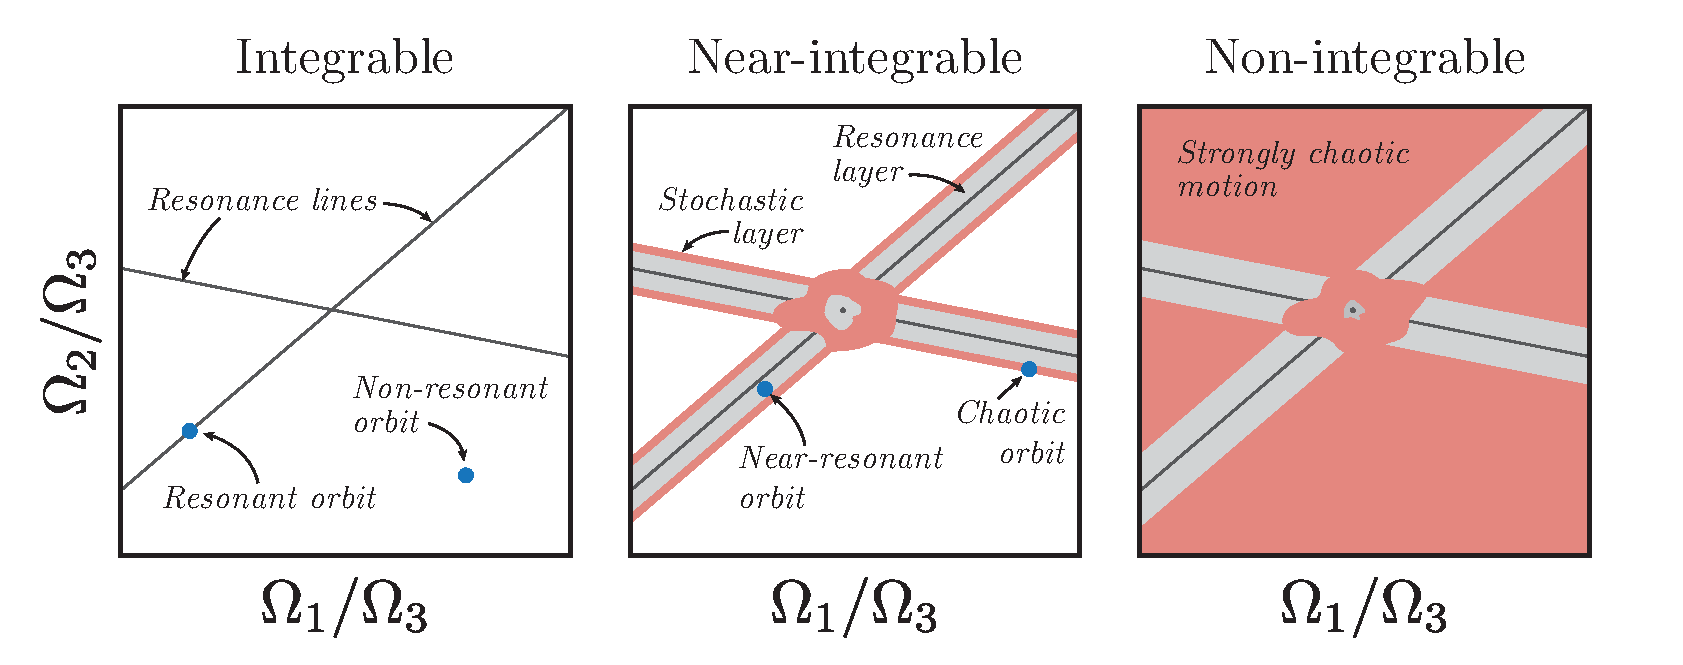
\includegraphics[width=\textwidth]{figures/cartoons.pdf}
\caption{} 
\label{fig:cartoons}
\end{center}
\end{sidewaysfigure}

% Figure ??
\begin{figure*}[!p]
\begin{center}
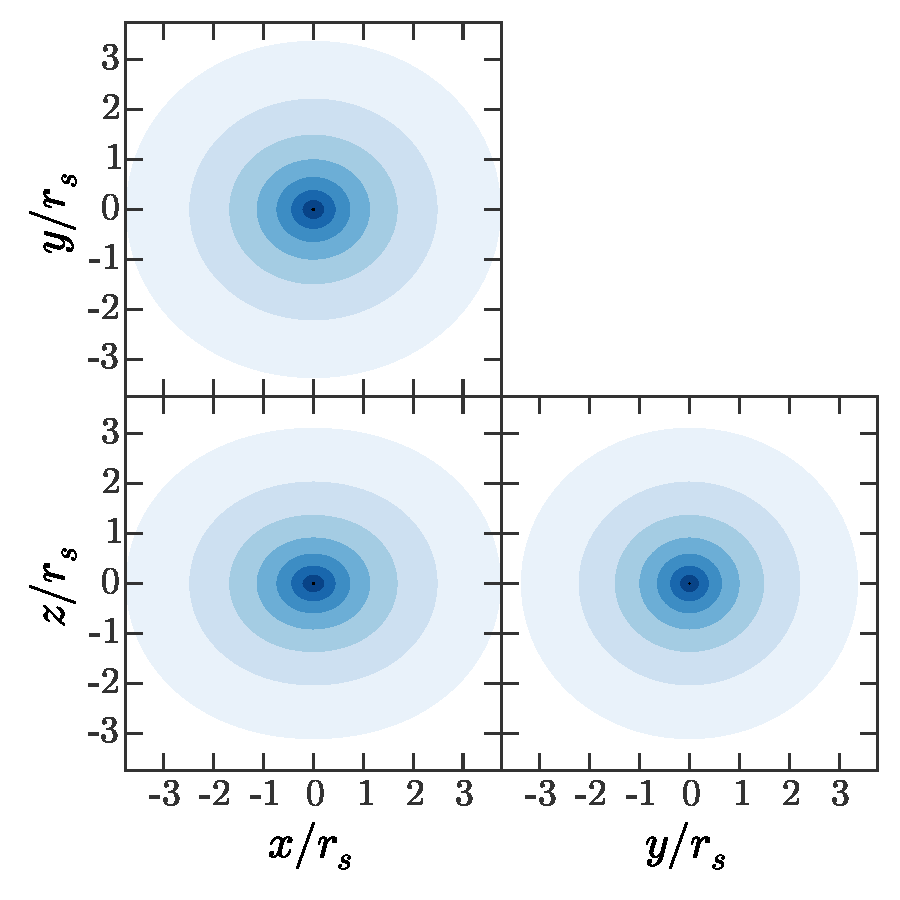
\includegraphics[width=\textwidth]{figures/potential.pdf}
\caption{Equipotential contours for the triaxial NFW potential considered in this work. There are eight contour levels evenly spaced and linear in the value of the potential. \todo{apw}{should I show density as well or instead?}} \label{fig:potential}
\end{center}
\end{figure*}

% Figure ??
\begin{figure*}[p]
\begin{center}
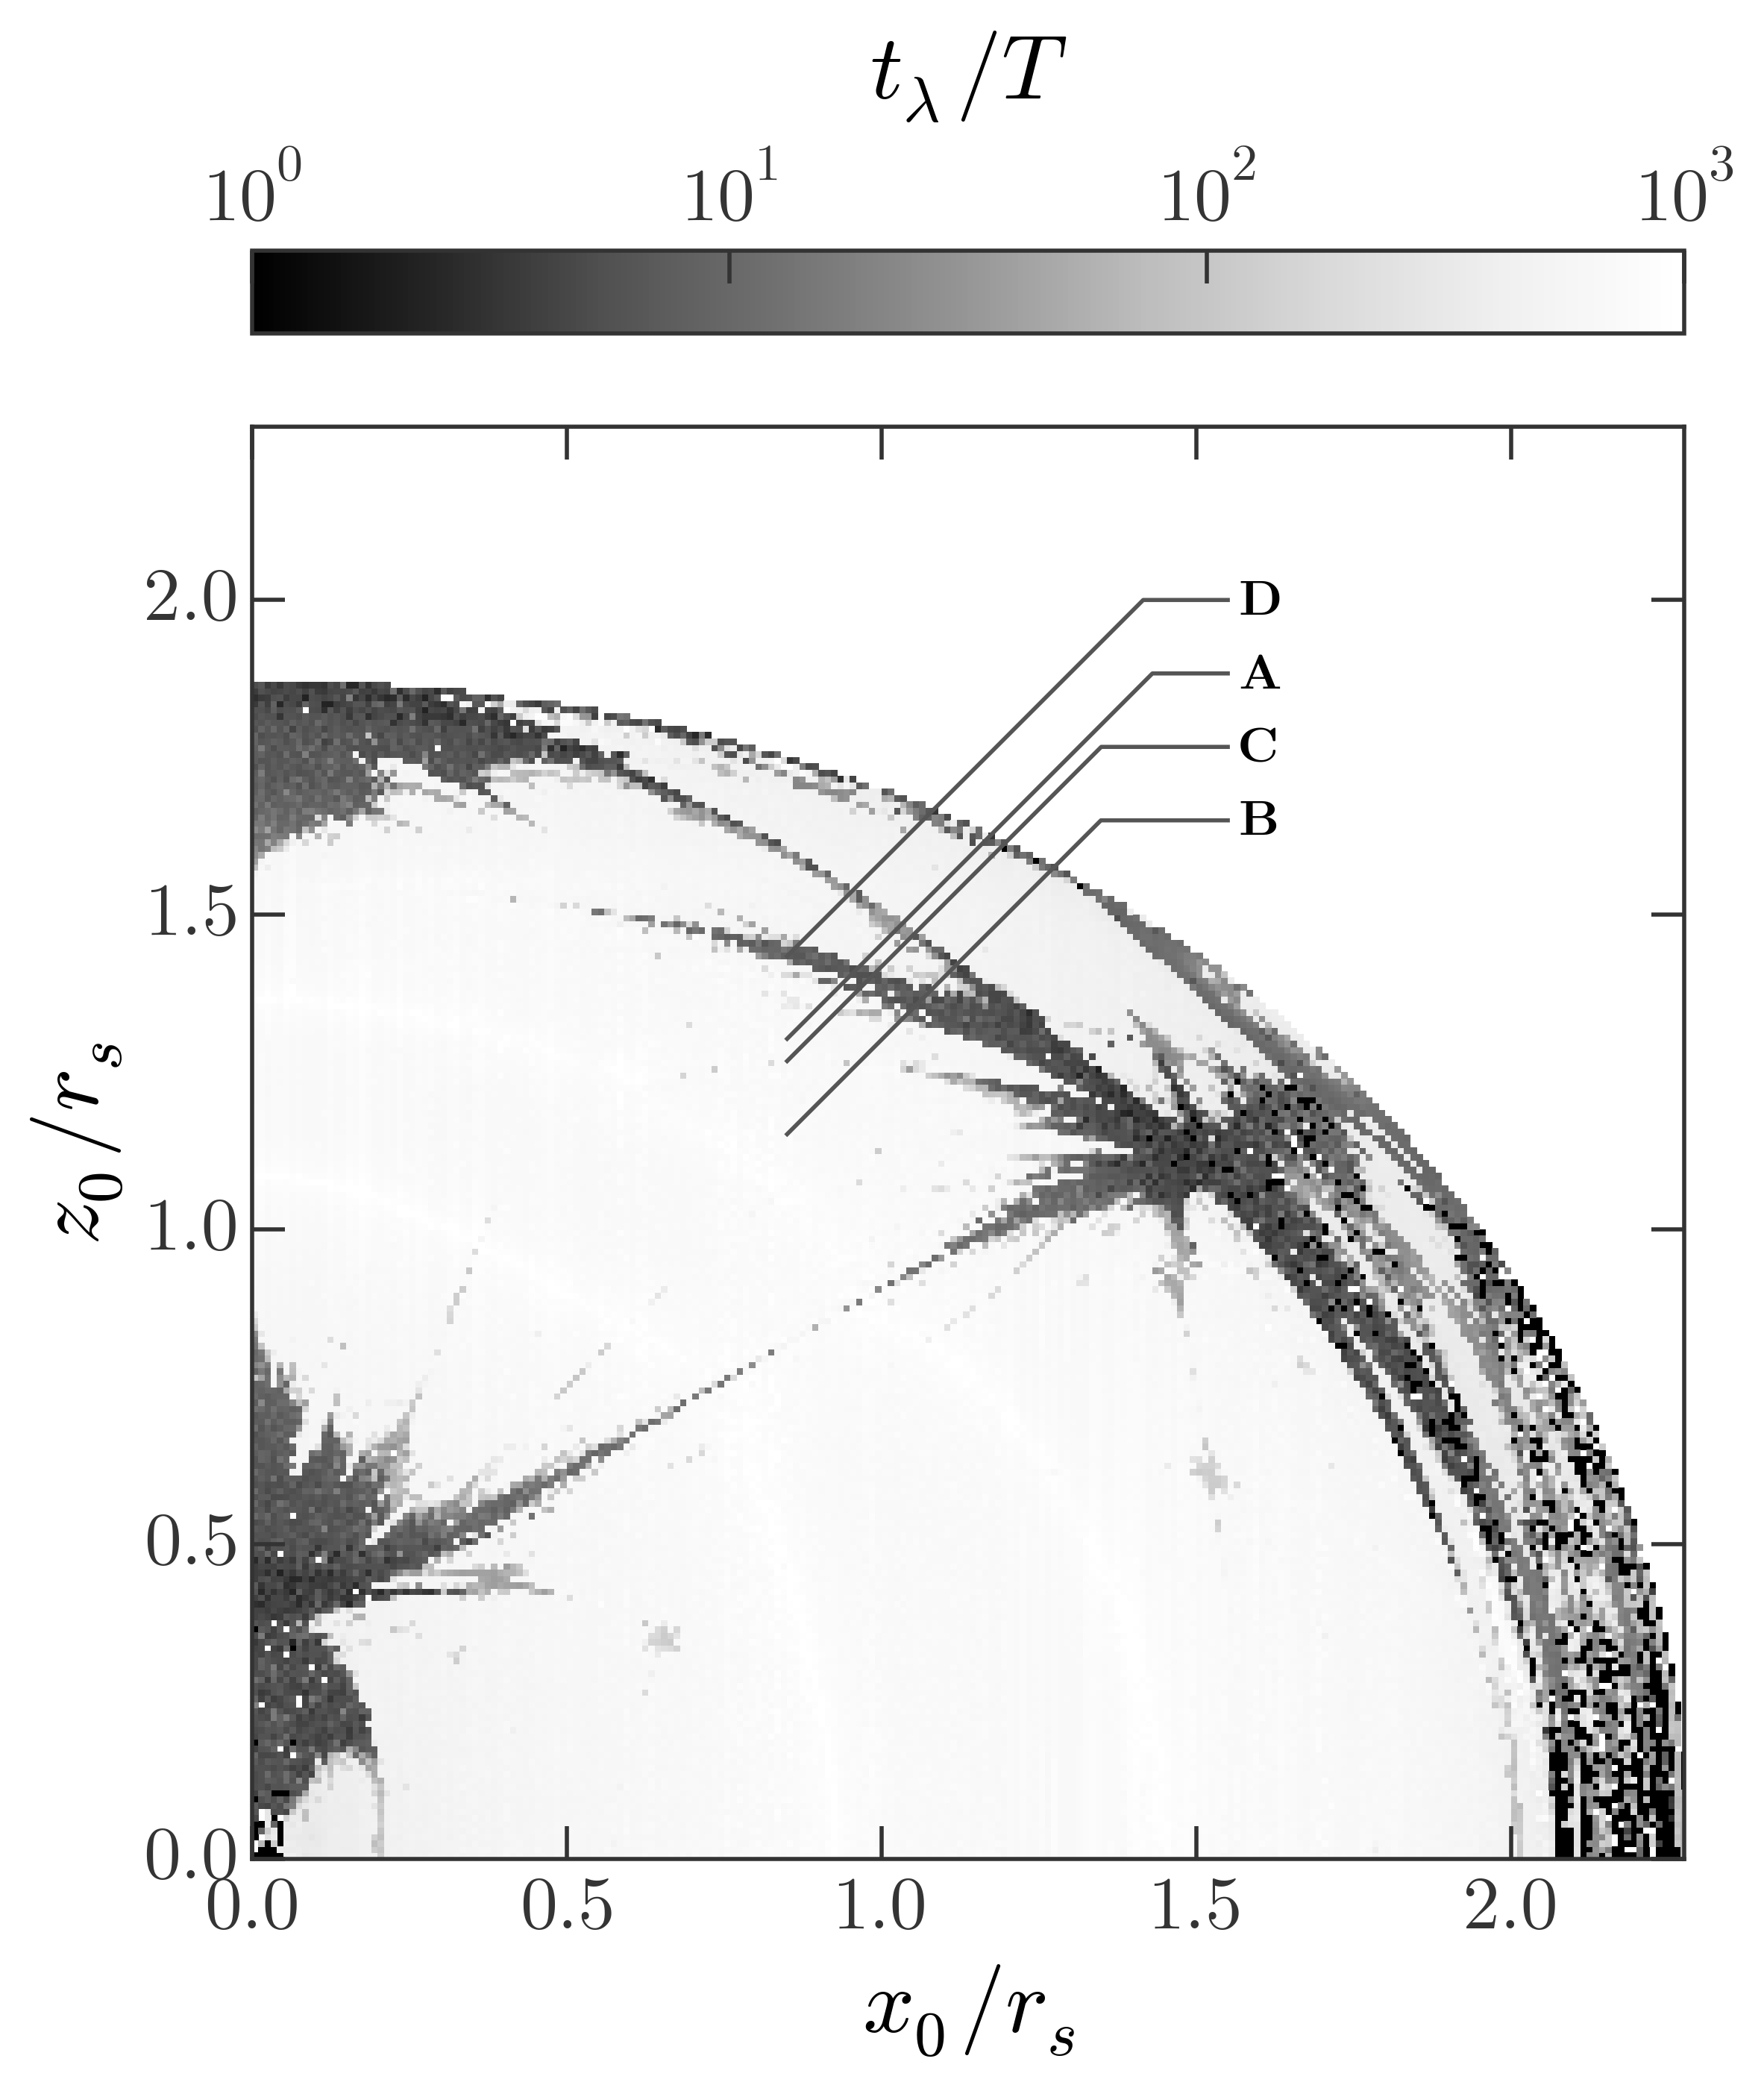
\includegraphics[width=\textwidth]{figures/lyap_map.png}
\caption{ A grid of isoenergy orbits initialized on the $xz$ plane. Each pixel in this image represents a single orbit, and the greyscale corresponds to the logarithm of the Lyapunov time (in units of orbital periods). Chaotic orbits with $t_\lambda \gtrsim XX~{\rm T}$ appear regular because the integration time for each orbit is insufficient to resolve weak chaos. \todo{apw}{remove Gyr and express in terms of orbital periods, add title, run Lyapunov grid for 5000 orbital periods instead of 1000?}} \label{fig:lyapmap} 
\end{center}
\end{figure*}

% Figure ??
\begin{figure*}[p]
\begin{center}
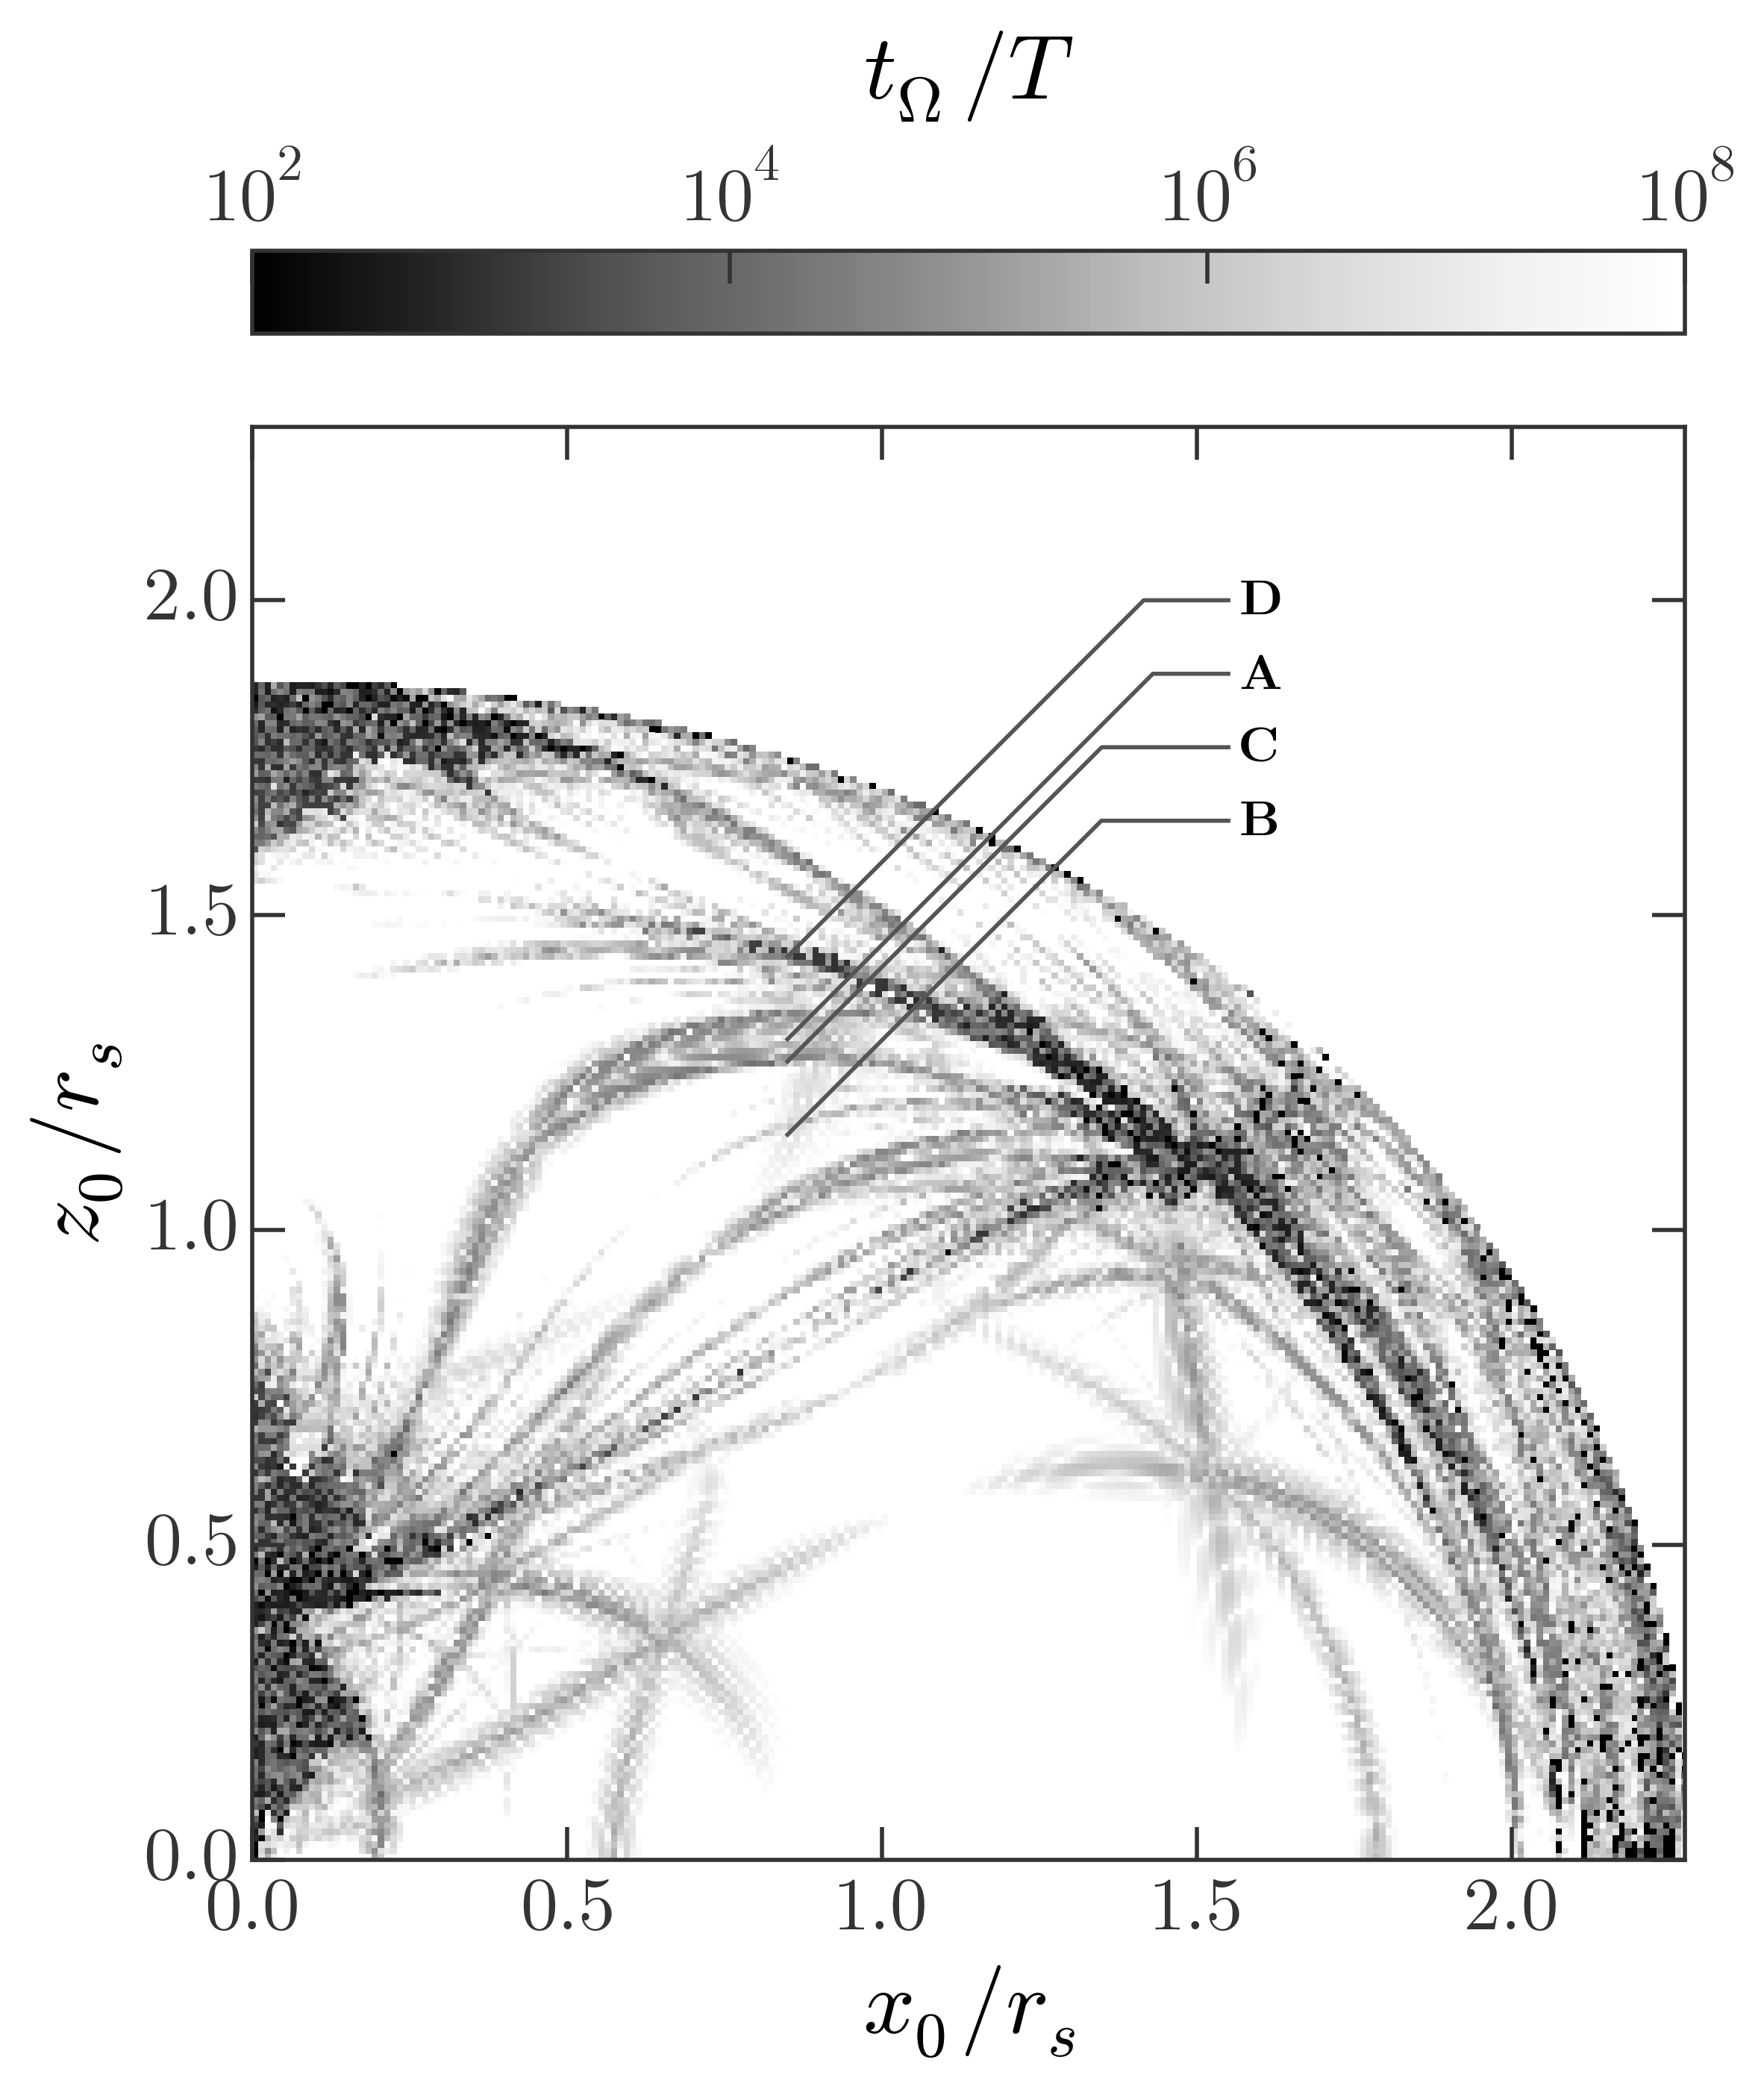
\includegraphics[width=\textwidth]{figures/fdiff_map.png}
\caption{The same grid of initial conditions as Figure~\ref{fig:lyapmap}, but now each pixel is colored by the logarithm of the frequency diffusion time (again in units of orbital periods). The frequencies are computed in two consecutive windows, each of which has length equal to 50 orbital periods. The frequencies are measured precisely so that small changes in the frequencies can be detected over just $\approx$10s of orbits. \todo{apw}{remove Gyr and express in terms of orbital periods, add title} } \label{fig:freqdiff}
\end{center}
\end{figure*}

% Figure ??
\begin{figure*}[p]
\begin{center}
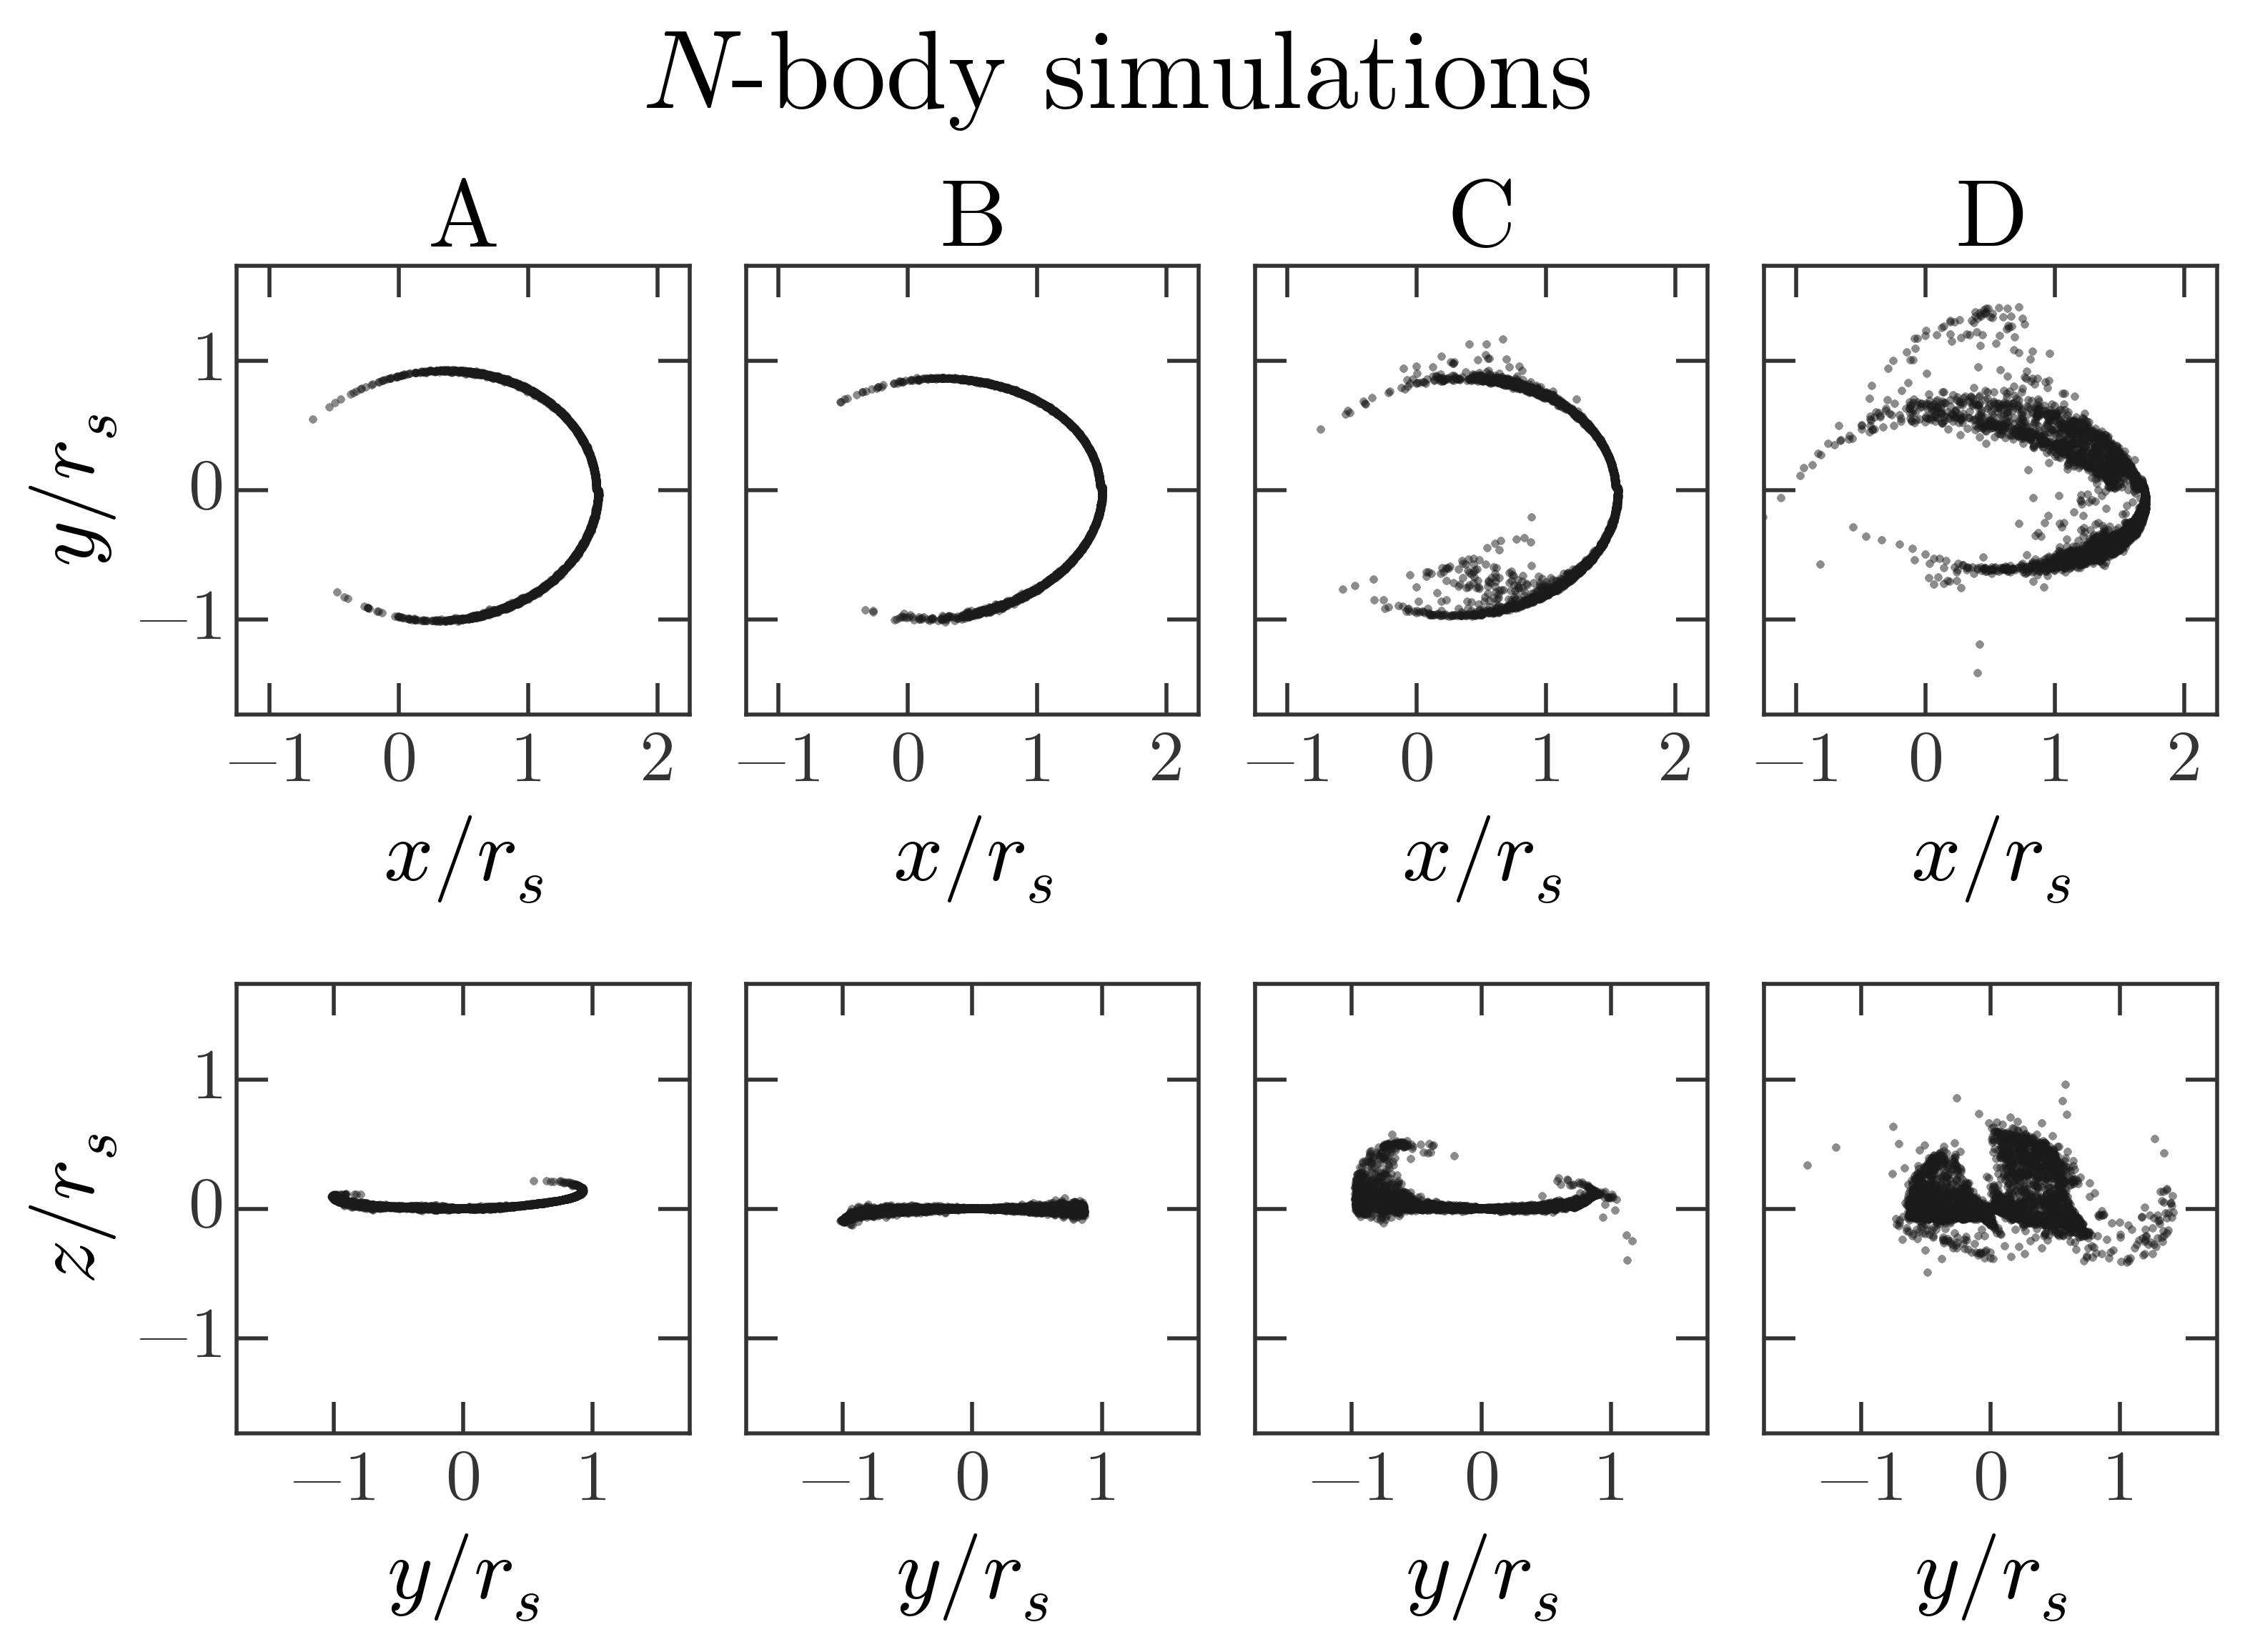
\includegraphics[width=\textwidth]{figures/nbody.png}
\caption{Particle positions from the final snapshots of N-body simulations of a globular-cluster-mass satellite disrupting in a triaxial NFW potential (Section~\ref{sec:potential}). Each satellite is evolved for 16 orbital periods, and begins and ends at apocenter. For visualization, the positions have been rotated so that the angular momentum of the progenitor at the final snapshot are aligned with the $z$-axis. Top row shows the positions projected onto the resulting $xy$ plane (the instantaneous orbital plane of the progenitor at the end of the simulation), bottom row shows the positions projected onto the $yz$ plane. From left to right, the columns indicate that the progenitor is on a regular (R), weakly chaotic (W), or strongly chaotic (S) orbit. Even on the weakly chaotic orbit --- where the predicted chaotic timescale is XX orbital periods --- the resulting tidal stream displays stream-fanning and the ``oldest'' debris is more diffuse than in the regular case. \todo{apw}{suptitle 'N-body simulations'?}} \label{fig:nbodysims}
\end{center}
\end{figure*}

% Figure ??
\begin{figure*}[p]
\begin{center}
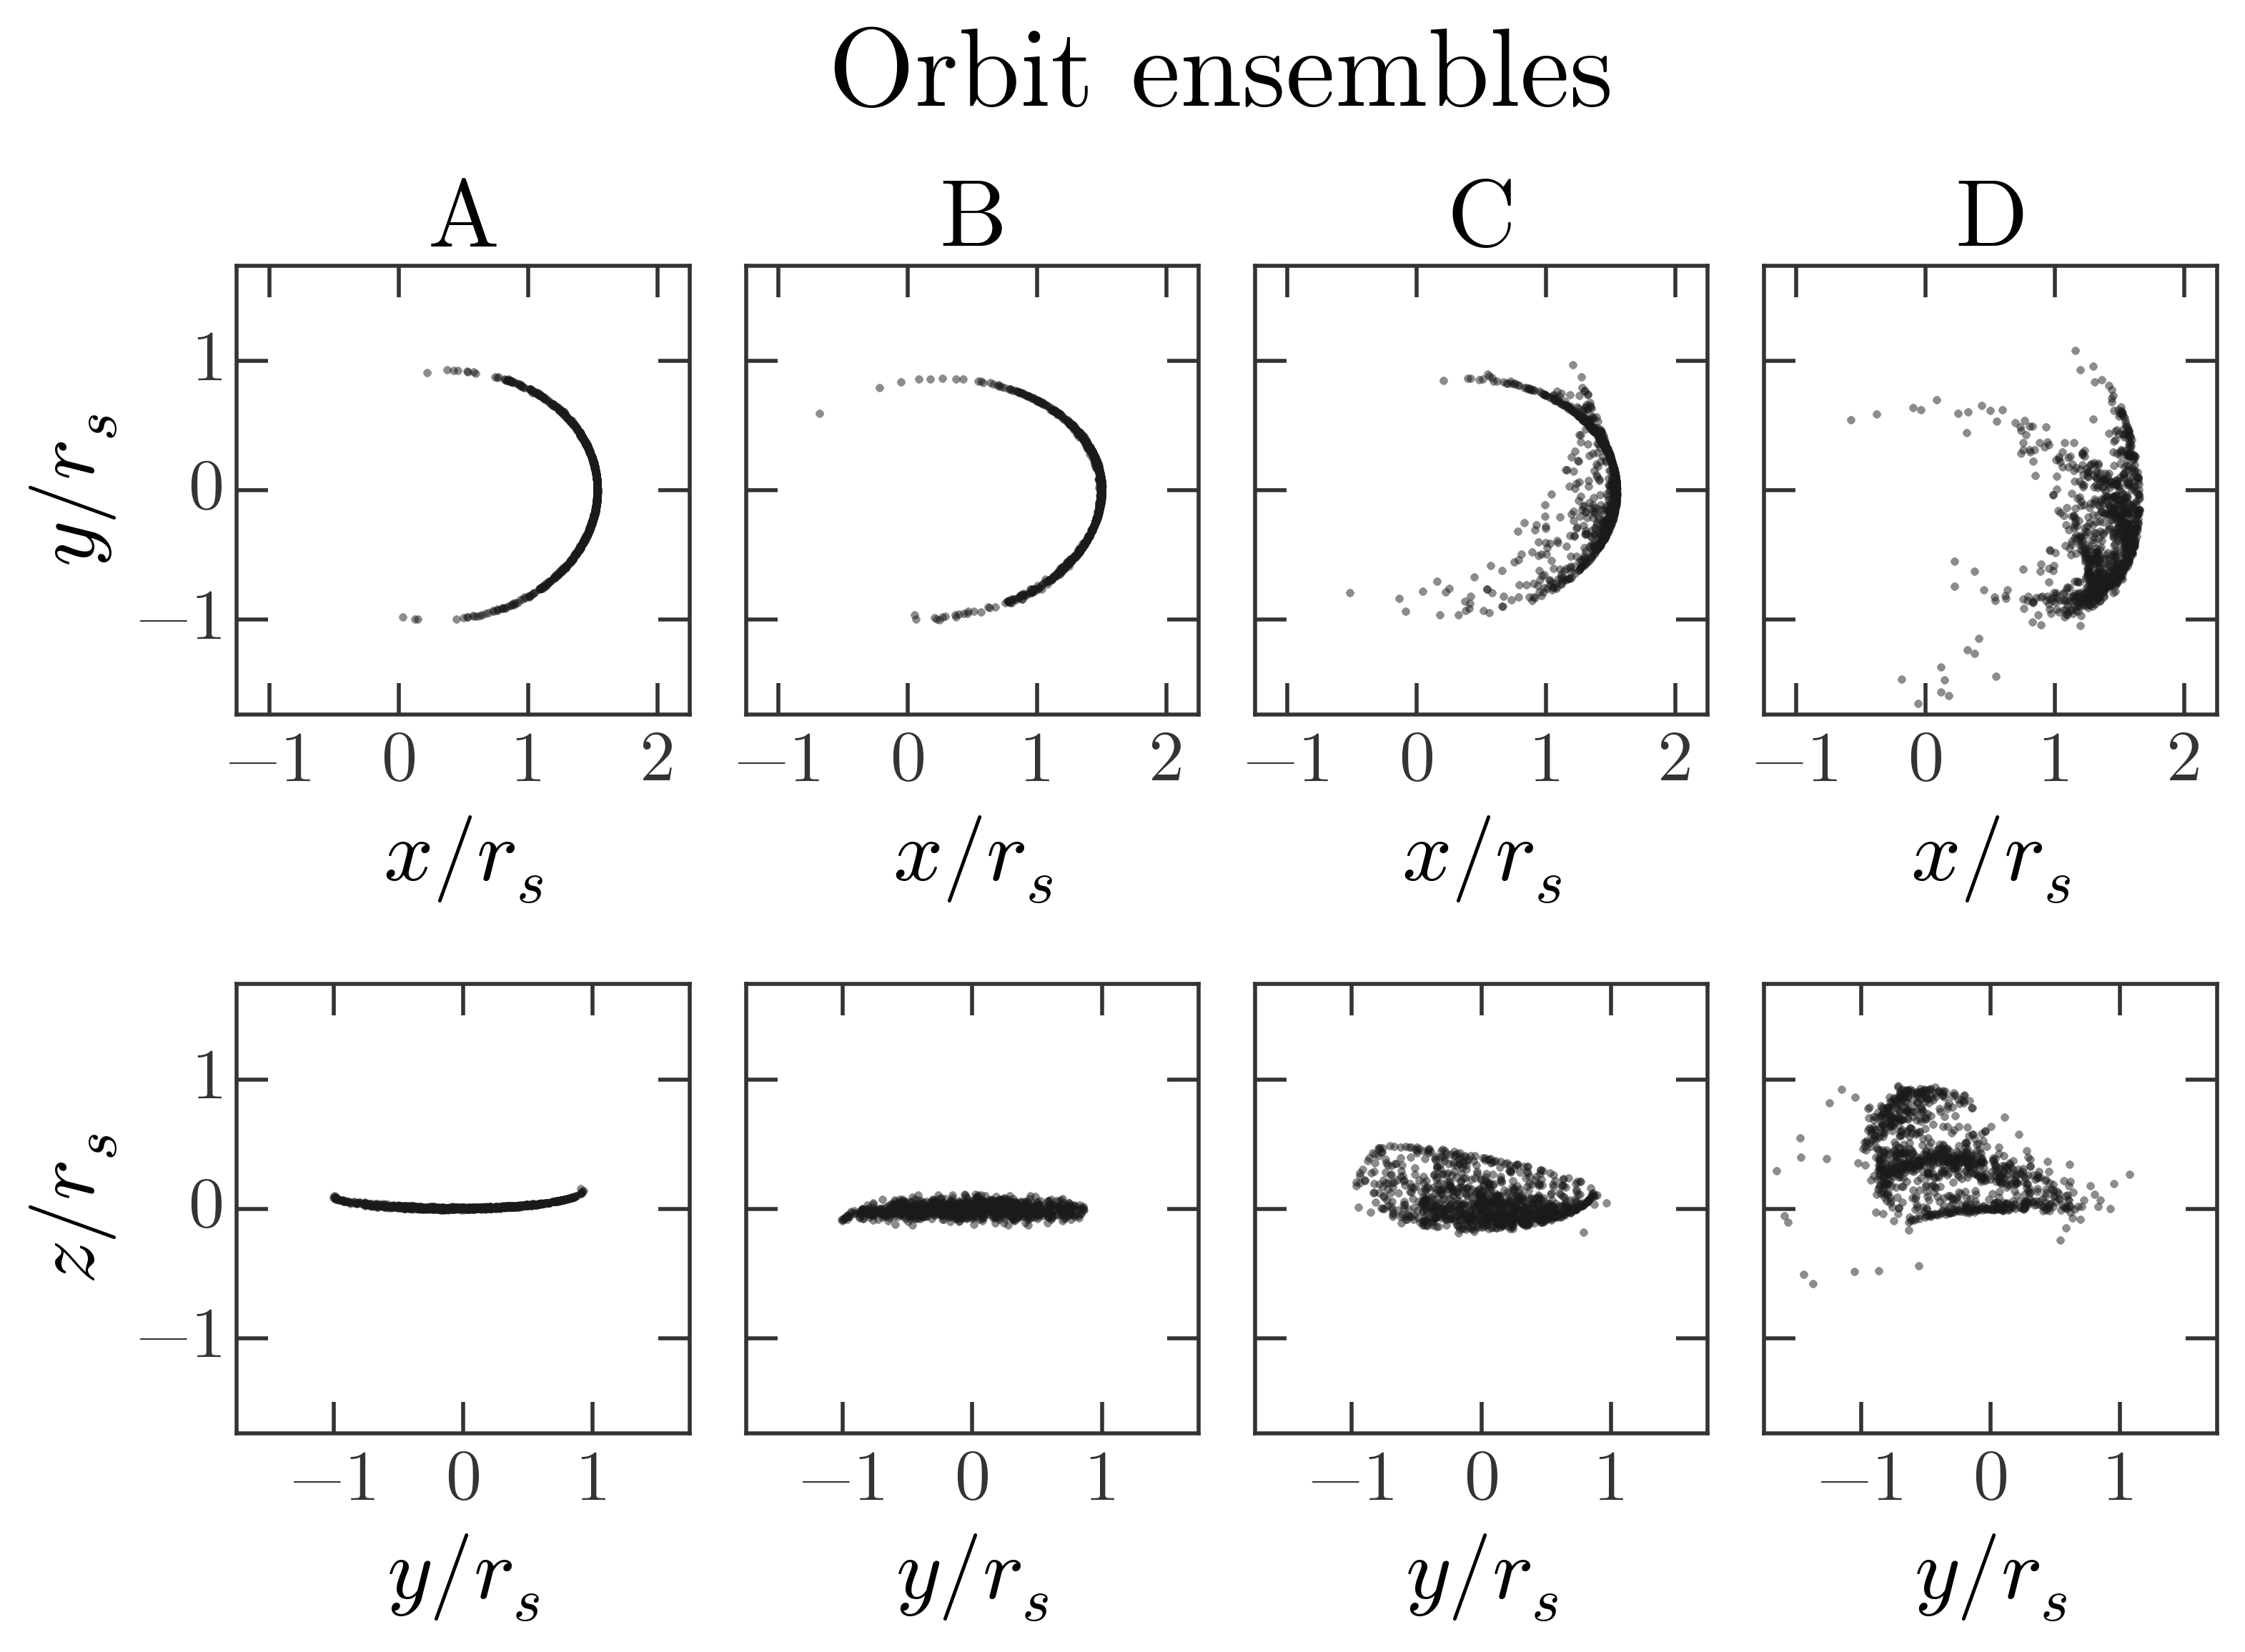
\includegraphics[width=\textwidth]{figures/ensembles.png}
\caption{Final particle positions after integrating unbound, globular-cluster-sized ensembles of orbits generated around each of the three N-body orbits (Figure~\ref{fig:nbodysims}). The ensembles each contain 1000 particles and begin at pericenter rather than apocenter because they are meant to represent debris disrupted during a single (the first) pericentric passage. The particle positions qualitatively match the morphology of the ``oldest'' debris from the N-body simulations, though there are many more particles in these ensembles than are disrupted during the first pericentric passage of the simulations. \todo{apw}{suptitle 'Orbit ensembles'?} } \label{fig:ensembles}
\end{center}
\end{figure*}

% Figure ??
\clearpage
\begin{figure*}[p]
\begin{center}
\includegraphics[width=\textwidth]{figures/ensemble-density.png}
\caption{ Distributions of the values of the estimated configuration-space density field evaluated at the positions of the ensemble particles after 4 (left), 8 (middle), and 16 (right) orbital periods. Colors represent the three orbits of Figures~\ref{fig:nbodysims} and \ref{fig:ensembles}: the regular, weakly chaotic, and strongly chaotic orbits. The density distribution of the regular orbit ensemble stays compact and decreases slowly. The density of the weakly chaotic ensemble initially evolves quickly to lower density, but then broadens. The strongly chaotic ensemble evolves fast to a state of low density. \todo{apw}{can't distinguish colors when printed...}} \label{fig:ensemble-density}
\end{center}
\end{figure*}

% Figure ??
\clearpage
\begin{figure*}[p]
\begin{center}
\includegraphics[width=\textwidth]{figures/ensemble-density-skewness.png}
\caption{ } \label{fig:density-skewness}
\end{center}
\end{figure*}

% Figure ??
\clearpage
\begin{figure*}[p]
\begin{center}
\includegraphics[width=\textwidth]{figures/ensemblemap-meandensity.png}
\caption{ } \label{fig:ensemblemap-meandensity}
\end{center}
\end{figure*}

% Figure ??
\clearpage
\begin{figure*}[p]
\begin{center}
\includegraphics[width=\textwidth]{figures/ensemblemap-skewness.png}
\caption{ } \label{fig:ensemblemap-skewness}
\end{center}
\end{figure*}

% Figure ??
\clearpage
\begin{figure*}[p]
\begin{center}
\includegraphics[width=1.1\textwidth]{figures/fdiff_zooms.png}
\caption{ } \label{fig:fdiff-zooms}
\end{center}
\end{figure*}

% Figure ??
\clearpage
\begin{figure*}[p]
\begin{center}
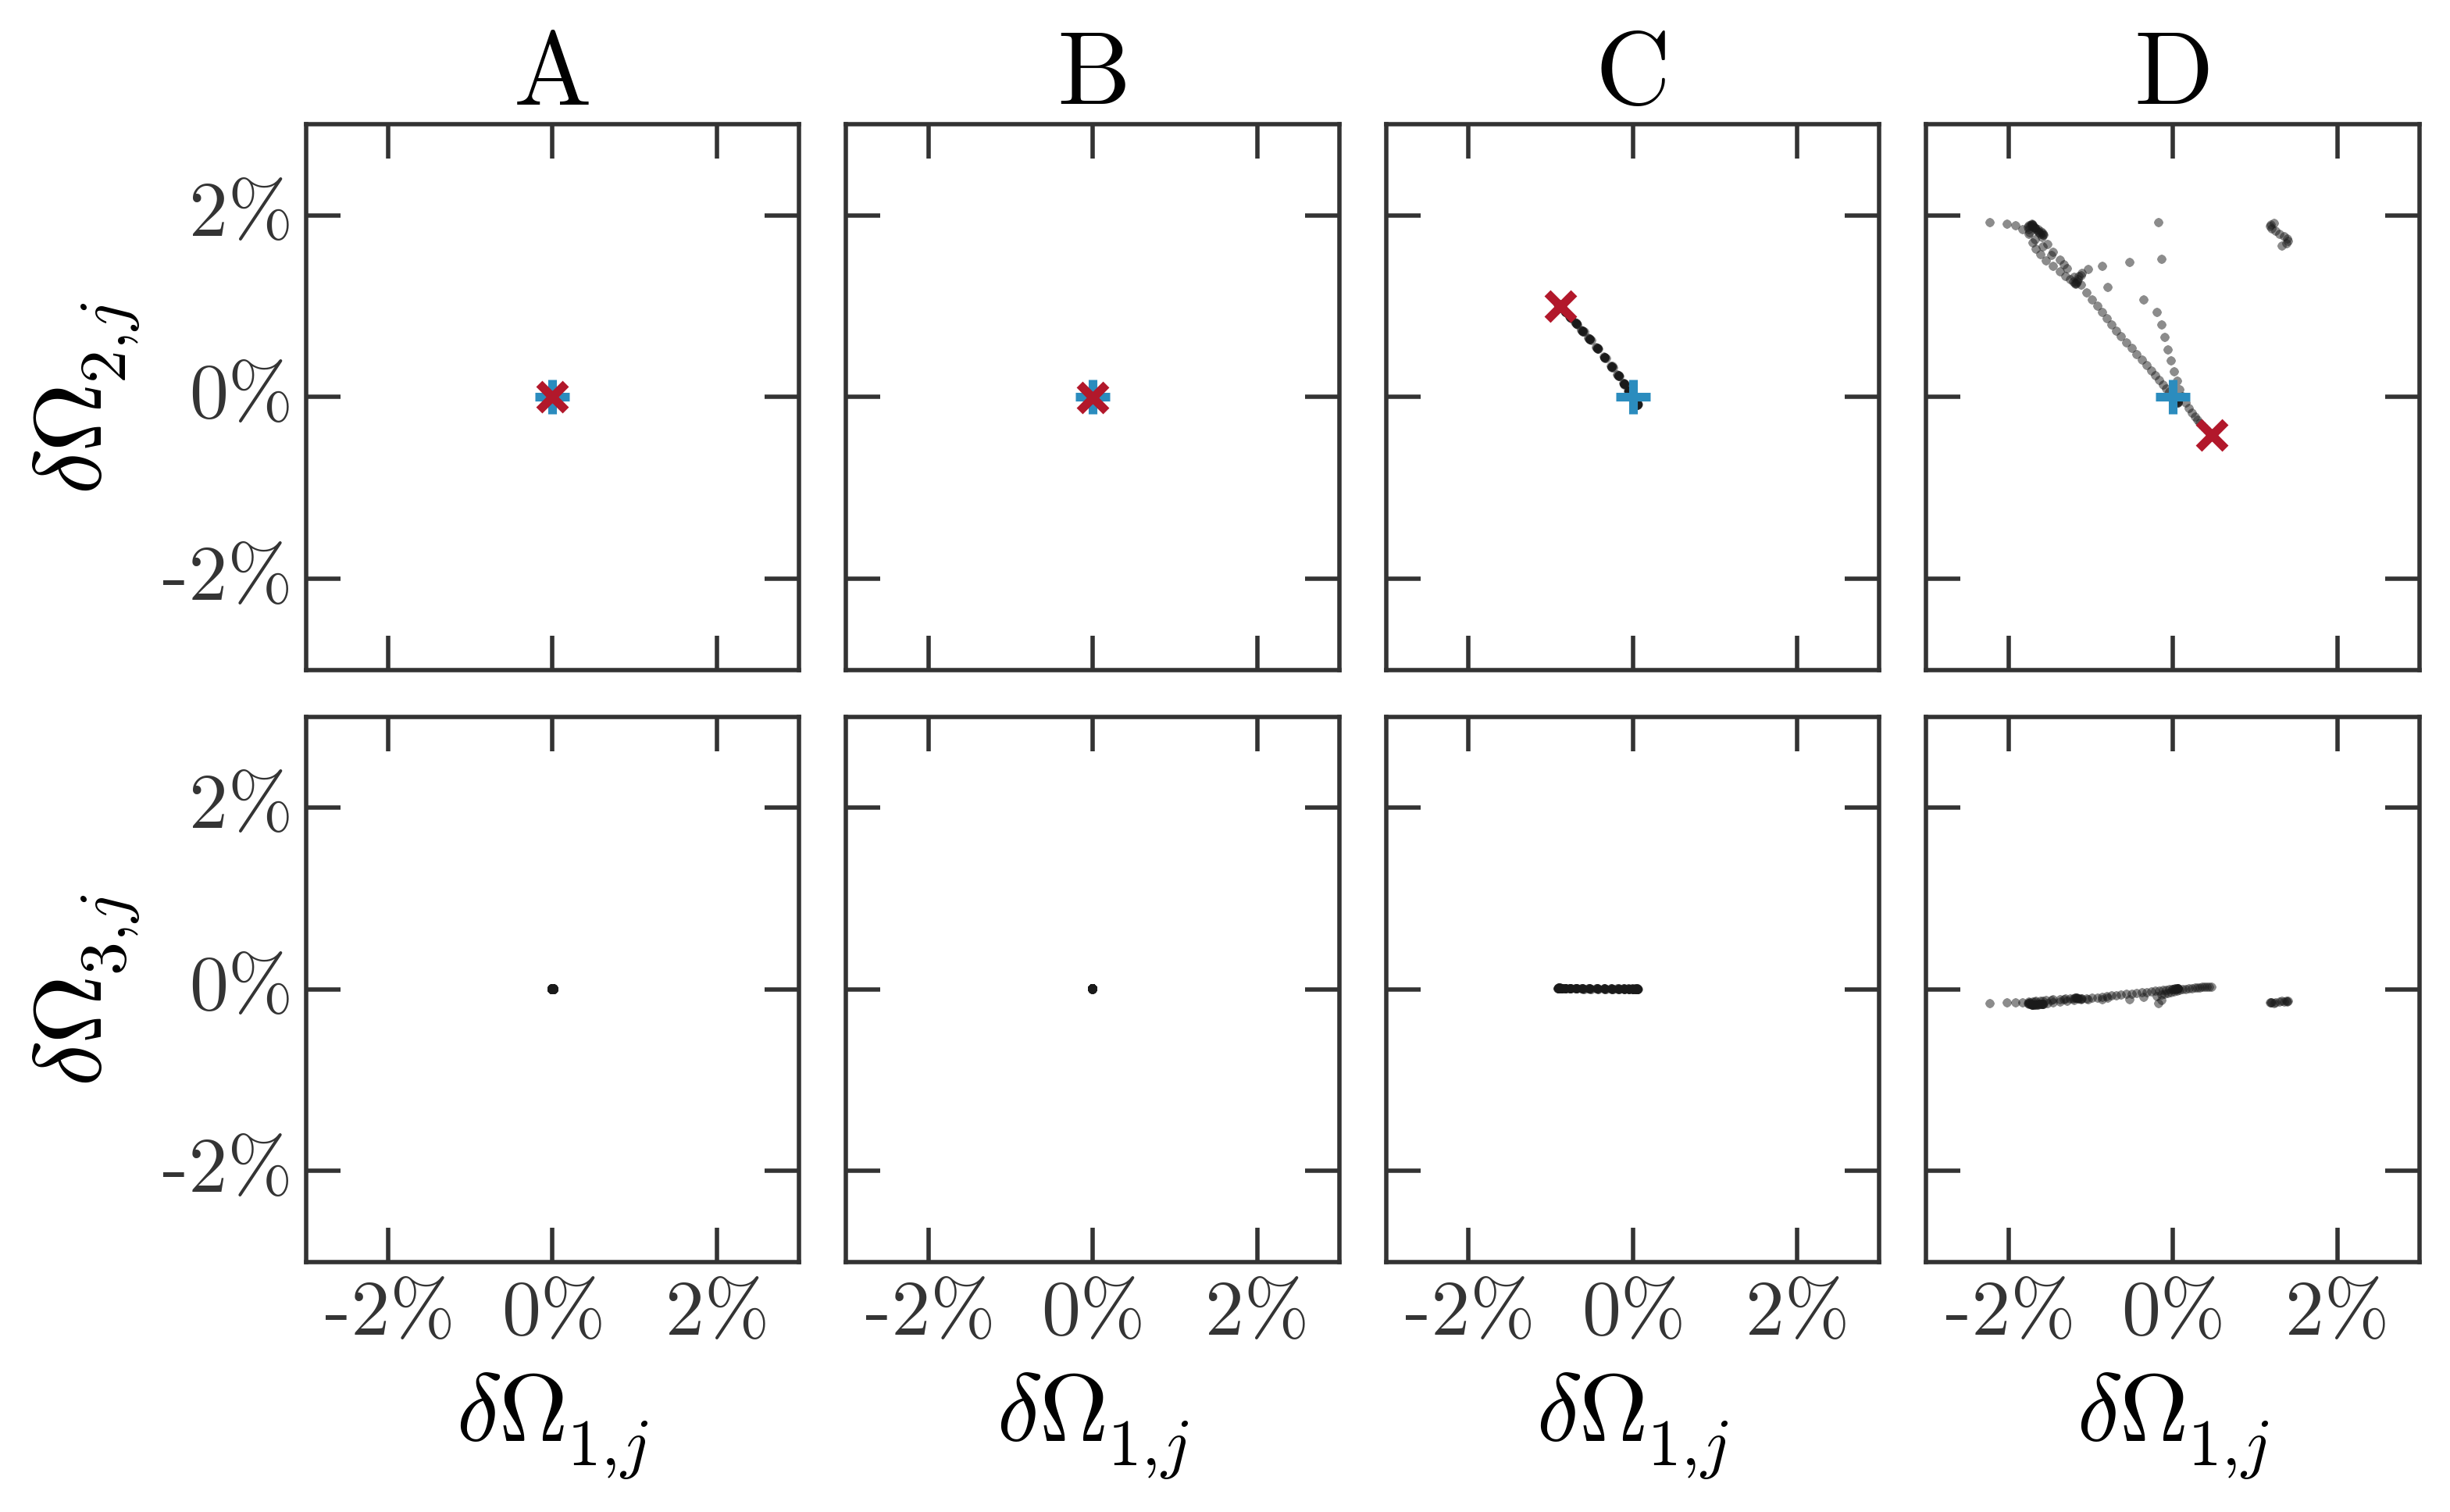
\includegraphics[width=\textwidth]{figures/freq-evolution.png}
\caption{ } \label{fig:three-orbits-freqs}
\end{center}
\end{figure*}

% Figure ??
\clearpage
\begin{figure*}[p]
\begin{center}
\includegraphics[width=\textwidth]{figures/freqvar.png}
\caption{ } \label{fig:freqvar_map}
\end{center}
\end{figure*}


\end{document}
